\documentclass[fr,license=none]{../../../eplexercises}
\usepackage{multido}
\usepackage{float}
\usepackage{../../../eplcode}
\usepackage{../../../eplunits}
\usepackage{listings}
\usepackage{booktabs}

% General info
\hypertitle[e ]{Systèmes informatiques 1}{3}{SINF}{1252}
{Brieuc Kaisin \and Cynthia Laureys \and Jean-Martin Vlaeminck}
{Olivier Bonaventure}
 
 
 % New colors
%\definecolor{codegreen}{rgb}{0,0.6,0}
%\definecolor{codegray}{rgb}{0.5,0.5,0.5}
%\definecolor{backcolour}{rgb}{0.95,0.95,0.92}

\lstdefinestyle{mystyle}{
    %backgroundcolor=\color{backcolour},
    %commentstyle=\color{codegreen},
    %keywordstyle=\color{RedViolet},
    %numberstyle=\tiny\color{codegray},
    %stringstyle=\color{red},
    %basicstyle=\footnotesize,
    %basicstyle=% change it if you want
    %    \ttfamily%
    %    \normalsize,
        %\lst@ifdisplaystyle\normalsize\fi,
    %breakatwhitespace=false,
    %breaklines=true,
    keepspaces=true,
    showspaces=false,
    showstringspaces=true,
    showtabs=false,
    tabsize=4 % nondidjou, ça vaut 4 ou 8 ! Pas 2 !
}


\lstset{style=mystyle, language=C}

%----------------------------------Macros--------------------------------------

\titleformat
{\section} % command
[display] % shape
{\bfseries\Large} % format
{\newpage Semaine \thesection} % label
{0.5ex} % sep
{} % before-code


\titleformat
{\subsection} % command
{\normalfont\large\bfseries} % format
{\thesubsection} % label
{0.5ex} % sep
{} % before-code

\newcommand\TODO{\textcolor{red}{TO DO}}
%\newcommand\question[1]{\medskip\noindent\subsubsection{Question #1}}
\newcommand{\question}[1]{\subsubsection{Question #1}}
\newcommand\ingi[2]{\begin{center}\textbf{#1}\\ \url{#2}\end{center}}
%\newcommand{\type}[1]{{\ttfamily\itshape#1}}
\newcommand\qcm[2]
{
	\multido{\i=1+1}{#2}{
    \begin{figure}[H]
    	\centering
        \includegraphics[width=14cm]{#1/Q\i.PNG}
    \end{figure}}
}
\renewcommand{\theQA}{\thesubsubsection}

%TODO insérer ces commandes dans un package externe, pouvant être utilisé par d'autres documents.
% Commande pour afficher les manpages. Modifier une seule fois pour changer le style des commandes une fois pour toute.
% xemple : \manpage[posix]{time}{1}, \manpage{signal}{2} ; il est nécessaire de mettre un \_ au lieu d'un _ (oui, ça marche dans href)
\newcommand{\manpage}[3][]{\href{https://sites.uclouvain.be/SystInfo/manpages/man#3/#2.#3#1.html}{#2(#3#1)}}
% Site de base où les programmes devront être affichés.
\newcommand{\basesourcelink}{https://sites.uclouvain.be/SystInfo/notes/Exercices/html/_downloads/}
% Insère un lien vers les programmes d'exemple utilisés dans les TP.
% Exemple : \sourcelink{/QCM/S7/src/}{pthread-mutex-perf.c}
% Affichera un lien indiquant "/QCM/S7/src/pthread-mutex-perf.c" chargeant la page https://sites.uclouvain.be/SystInfo/notes/Exercices/html/_downloads/pthread-mutex-perf.c
% FIXME rendre cette commande un peu plus générale
\newcommand{\sourcelink}[3][\basesourcelink]{\href{#1#3}{#2#3}}
% Affiche un chemin de fichier ; changez le style à votre guise
\newcommand{\filepath}[1]{\texttt{#1}}
% Affiche une ligne de commande bash ; changez le style à votre guise. Si vous avez des bugs car vous avez trouvé une commande avec un point d'exclamation, vous savez quoi corriger.
\newcommand{\cmdline}[1]{
	\lstinline[%
		language=bash,%
		literate={\$\#}{{{\$\#}}}2
	]!#1!}

%------------------------------------------------------------------------------   

\section*{Remarques importantes}

Ceci est un \og correctif\fg{} des exercices des séances de TP du cours de systèmes informatiques.
Il a été réalisé par les étudiants mentionnés sur la première page, avec l'aide des autres étudiants.
Sa réalisation a été motivée par l'absence de correctif officiels pour les exercices du cours,
ainsi que par les corrections souvent incomplètes effectuées lors des séances de TP
(manque de temps pour réaliser tous les exercices prévus).
Ce correctif a pour but de proposer des bases de solutions, suffisamment claires que pour pouvoir être utilisées lors de la préparation de l'examen, et comble le manque de correctif.

Pour ce cours, probablement plus que pour les autres, il est \strong{indispensable} d'effectuer les exercices des séances par soi-même :
la matière de ce cours ne s'apprend qu'en participant activement au cours et en résolvant tous les exercices.
Vous n'apprendrez rien si vous vous contentez de lire les réponses proposées par d'autres étudiants,
sans tenter s'approprier leur code en faisant des tests et en explorant les possibilités.
Vous n'apprendrez rien si vous ne pratiquez pas le langage C ni tous les concepts vus au cours.

Dès lors, ne lisez pas les corrections proposées dans ce document avant d'avoir réellement essayé de résoudre l'exercice,
et de vous être fait insulté de nombreuses fois par le compilateur (sauf si vous résolvez les exercices rapidement).
Ne lisez pas ces corrections avant ou pendant la séance, mais uniquement après, pour comparer vos réponses avec celles-ci ;
vous aurez ainsi une confirmation de vos connaissances ainsi qu'un autre point de vue sur les exercices.

Après chaque séance, terminez celle-ci en effectuant les exercices non abordés durant le TP :
chaque exercice a sa valeur et son utilité.

Encore une chose : les solutions proposées ici proviennent d'étudiant qui, comme vous, n'ont pas eu le temps de faire tous les exercices en séance
et ont dû se débrouiller pour obtenir des solutions à peu près réalistes.
Il est donc probable, et quasiment certain, qu'il y ait des imprécisions, des oublis, des erreurs voire du grand n'importe quoi.
Prenez toutes ces corrections avec des pincettes et, si vous trouvez des erreurs,
n'hésitez pas à les rapporter sur le Github du projet (première page).

Pour ce qui est des réponses aux QCM (qui sont conçus pour vous permettre de vous évaluer : ça ne sert à rien de regarder la solution en les faisant),
celles-ci peuvent se trouver sur
\begin{center}
	\url{https://github.com/obonaventure/SystemesInformatiques/tree/master/Exercices/QCM}
\end{center}
Vous naviguez jusqu'au bon QCM (un fichier .rst), vous l'affichez en \og Raw\fg{}, et les bonnes réponses sont marquées par l'indication \og positive \fg{}.


%--------------------------------------S1--------------------------------------
\section{Introduction à Unix et au langage C} %1
\pagenumbering{arabic}
\subsection{QCM}
%\qcm{QCMS1}{5}

\subsection{Exercices en bash}
\TODO

\subsection{Questions de base}
\question{1,2,6}
\begin{description}
\item[-Werror] Make all warnings into errors.
\item[-Wall] This enables all the warnings about constructions that some
users consider questionable, and that are easy to avoid (or modify to
prevent the warning), even in conjunction with macros. This also enables
some language-specific warnings described in C++ Dialect Options and
Objective-C and Objective-C++ Dialect Options.
\item[(-Wfatal-errors] This option causes the compiler to abort compilation
on
the first error occurred rather than trying to keep going and printing further
error messages.)
\end{description}

\question{3,7} Il faut rajouter \textit{return 0;} par exemple.

\question{8}
\url{http://sites.uclouvain.be/SystInfo/manpages/man3/atoi.3.html}\\
\url{http://sites.uclouvain.be/SystInfo/manpages/man3/strtol.3.html}

\question{9} EASY

\question{10} \TODO

\subsection{Petits programmes}

\question{1} \url{http://sites.uclouvain.be/SystInfo/manpages/man1/test.1.html}
\ingi{La commande test}{https://inginious.info.ucl.ac.be/course/LSINF1252/commandetest}
\begin{lstlisting}
#include <stdlib.h>
#include <stdio.h>
#include <string.h>

int eq(int n1, int n2)
{
	if(n1 == n2)
	return 0;
	else
	return 1;
}
int ge(int n1, int n2)
{
	if(n1 >= n2)
	return 0;
	else
	return 1;
}
int gt(int n1, int n2)
{
	if(n1 > n2)
	return 0;
	else
	return 1;
}
int le(int n1, int n2)
{
	if(n1 <= n2)
	return 0;
	else
	return 1;
}
int lt(int n1, int n2)
{
	if(n1 < n2)
	return 0;
	else
	return 1;
}
int ne(int n1, int n2)
{
	if(n1 != n2)
	return 0;
	else
	return 1;
}

int main(int argc, char *argv[])
{
	if(argc == 4)
	{
		int n1 = atoi(argv[1]);
		int n2 = atoi(argv[3]);
		
		if(strcmp(argv[2],"-eq") == 0)
			return eq(n1,n2);
		else if(strcmp(argv[2],"-ge") == 0)
			return ge(n1,n2);
		else if(strcmp(argv[2],"-gt") == 0)
			return gt(n1,n2);
		else if(strcmp(argv[2],"-le") == 0)
			return le(n1,n2);
		else if(strcmp(argv[2],"-lt") == 0)
			return lt(n1,n2);
		else if(strcmp(argv[2],"-ne") == 0)
			return ne(n1,n2);
		else
		printf("bad instruction ");
	}
	else
	{
		printf("Incorrect number of arguments (%d argument(s))\n",argc);
	}
	return 1;
}
\end{lstlisting}

\question{2} Fort semblable à la question 1.\\
\url{http://sites.uclouvain.be/SystInfo/manpages/man1/expr.1.html}

\question{3} \TODO

%--------------------------------------S2--------------------------------------
\section{Types de données} %2
\subsection{QCM}
%\qcm{QCMS2}{13}

\subsection{Questions de base}
\question{1}
\begin{lstlisting}
#include <stdio.h>
#include <stdint.h>

int main(int argc, const char *argv[])
{
    printf("int : %d bytes\n", sizeof(int));
    printf("long : %d bytes\n", sizeof(long));
    printf("void* : %d bytes\n", sizeof(void *));
    printf("char* : %d bytes\n", sizeof(char *));
    printf("size_t : %d bytes\n", sizeof(size_t));
    printf("uint64_t : %d bytes\n", sizeof(uint64_t));
}
\end{lstlisting}

\question{2}
\begin{lstlisting}
void lsb(int number)
{
    int nbr = number;
    int bit = 32;
    while (nbr!=0)
    {
        nbr<<=1;
        bit--;
        //amelioration : effectuer bit-- avec des operations binaires
    }
    printf("Less significant bit of %d : %d", number, (int) pow(2,bit));
}
\end{lstlisting}

\question{3}
\begin{lstlisting}
#include <stdio.h>

int main()
{
    char* ptr = "Test";
    int i;
    for (i=0 ; i<4 ; i++){
        printf("%p\n", (void *) (ptr+i)); //or &ptr[i]
    }
}
\end{lstlisting}

\question{4}
\ingi{Echange de valeurs de fractions}{https://inginious.info.ucl.ac.be/course/LSINF1252/swap}
\begin{lstlisting}
void swap(struct fract_t *a, struct fract_t *b)
{
    int mem1 = a->num;
    int mem2 = a->denum;
    a->num = b->num;
    a->denum = b->denum;
    b->num = mem1;
    b->denum = mem2;
}
\end{lstlisting}

\question{5}
\begin{lstlisting}
#include <stdio.h>

int main()
{
    struct foo_t
    {
        char a;
        int b;
    };
    printf("Size of struct foo_t : %d bytes",sizeof(struct foo_t));
}
\end{lstlisting}

L'exécution de ce code affiche : \lstinline{Size of struct foo\_t : 8 bytes} et non 5 bytes (1+4) comme on pourrait le penser. Cela est dû à un phénomène d'alignement sur 32 bits du \textit{char a}.

\question{6}
\url{http://sites.uclouvain.be/SystInfo/manpages/man3/string.3.html}\\
\url{http://sites.uclouvain.be/SystInfo/manpages/man3/strlen.3.html}\\
\url{http://sites.uclouvain.be/SystInfo/manpages/man3/strcat.3.html}\\
\url{http://sites.uclouvain.be/SystInfo/manpages/man3/strcasecmp.3.html}\\
\textcolor{red}{Avertissement : ce code n'a pas encore été testé sur inginious (nombre d'essais limité)}

\ingi{Mini-projet : implémentation de strlen, strcat et strcasecmp}{https://inginious.info.ucl.ac.be/course/LSINF1252/mini-projet-string}
\begin{lstlisting}
size_t strlen(const char *str) {
    int i;
    for(i=0 ; str[i]!='\0';i++);
    return (size_t) i;
}

char *strcatt(char *destination, const char *source) {
    int i;
    int lenD = strlen(destination);
    int lenS = strlen(source);
    for (i=lenD ; i<lenD+lenS ; i++)
    {
        destination[i] = source[i-lenD];
    }
    destination[i+1] = '\0';
    return destination;
}

int strcasecmp(const char *s1, const char *s2) {
//TO DO
}
\end{lstlisting}

%--------------------------------------S3--------------------------------------
\section{Organisation de la mémoire} %3
\subsection{QCM}
%\qcm{QCMS3}{7}

\subsection{Questions}

\question{1}
\begin{description}
\item[void *calloc(size\_t nmemb, size\_t size);] allocates memory for an array of
\textit{nmemb} elements of size bytes each and returns a pointer to the allocated
memory. The memory is set to zero. If \textit{nmemb} or size is 0, then
\textit{calloc()} returns either NULL, or a unique pointer value that can later be
successfully passed to \textit{free()}.
\item[void *malloc(size\_t size);] allocates \textit{size} bytes and returns a pointer
to the allocated memory. The memory is not cleared. If size is 0, then
\textit{malloc()} returns either NULL, or a unique pointer value that can later be
successfully passed to \textit{free()}.
\item[void free(void *ptr);] frees the memory space pointed to by \textit{ptr}, which
must have been returned by a previous call to \textit{malloc()}, \textit{calloc()} or
\textit{realloc()}. Otherwise, or if \textit{free(ptr)} has already been called
before, undefined behavior occurs. If ptr is NULL, no operation is performed.
\item[void *realloc(void *ptr, size\_t size);] changes the size of the memory block
pointed to by \textit{ptr} to \textit{size} bytes. The contents will be unchanged to
the minimum of the old and new sizes; newly allocated memory will be uninitialized. If
\textit{ptr} is NULL, then the call is equivalent to \textit{malloc(size)}, for all
values of \textit{size}; if \textit{size} is equal to zero, and \textit{ptr} is not
NULL, then the call is equivalent to \textit{free(ptr)}. Unless \textit{ptr} is NULL,
it must have been returned by an earlier call to \textit{malloc()}, \textit{calloc()}
or \textit{realloc()}. If the area pointed to was moved, a \textit{free(ptr)} is done.
\end{description}
\textit{calloc()} est plus lent que \textit{malloc()}.

\question{2} \TODO
\begin{lstlisting}
/**************************************
 * stack.c
 *
 * Programme d'exemple implementant un stack comme structure
 * chainee
 *
 **************************************/

#include <stdio.h>
#include <stdlib.h>

typedef struct fraction_t {
  int num;
  int den;
} fraction;

///AAA
typedef struct node_t
{
  struct fraction_t *data;
  struct node_t *next;
} node;

struct node_t *stack; // sommet de la pile

// ajoute un element au sommet de la pile
void push(struct fraction_t *f)
{
  struct node_t *n;
  n=(struct node_t *)malloc(sizeof(struct node_t));
  if(n==NULL)
    exit(EXIT_FAILURE);
  n->data = f;
  n->next = stack;
  stack = n;
}
// retire l'element au sommet de la pile
struct fraction_t * pop()
{
  if(stack==NULL)
    return NULL;
  // else
  struct fraction_t *r;
  struct node_t *removed=stack;
  r=stack->data;
  stack=stack->next;
  free(removed);
  return (r);
}

///BBB

// affiche le contenu de la pile
void display()
{
  struct node_t *t;
  t = stack;
  while(t!=NULL) {
    if(t->data!=NULL) {
      printf("Item at addr %p  :  Fraction %d/%d   Next %p\n",t,t->data->num,t->data->den,t->next);
    }
    else {
      printf("Bas du stack %p\n",t);
    }
    t=t->next;
  }
}

// exemple
int main(int argc, char *argv[]) {

  struct fraction_t demi={1,2};
  struct fraction_t tiers={1,3};
  struct fraction_t quart={1,4};
  struct fraction_t zero={0,1};

  // initialisation
  stack = (struct node_t *)malloc(sizeof(struct node_t));
  stack->next=NULL;
  stack->data=NULL;

  display();
  push(&zero);
  display(); %splay()
  push(&demi);
  push(&tiers);
  push(&quart);
  display();

  struct fraction_t *f=pop();
  if(f!=NULL)
    printf("Popped : %d/%d\n",f->num,f->den);

  return(EXIT_SUCCESS);
}
///CCC
\end{lstlisting}

\question{3}
\TODO

\question{4}
\TODO

\question{5}
\begin{lstlisting}
int main()
{
    int i;
    int a[3][3] = { {1,2,3} , {4,5,6} , {7,8,9} };
    int *b = &a;
    for(i=0 ; i<9 ; i++) printf("%d\n",*b+i);
    return 0;
}
\end{lstlisting}
Le programme affiche \textit{1,2,3,4,5,6,7,8,9}. Conclusion : le tableau \textit{a} est stocké ligne par ligne.

\question{6}
\begin{lstlisting}
int main()
{
    typedef struct
    {
        char c;
        long l;
        short s;
    } test_t;
    printf("Size of struct test_t : %d bytes",sizeof(test_t));
    return 0;
}
\end{lstlisting}
Le programme indique que la taille de la structure vaut 12 bytes.

\begin{lstlisting}
int main()
{
    typedef struct
    {
        char c;
        long l;
        short s;
    } test_t;
    test_t stru;
    stru.c = 4;
    stru.l = 456;
    stru.s = 42;
    int* ptrC = &stru.c;
    int* ptrL = &stru.l;
    int* ptrS = &stru.s;
    printf("%p, %p, %p",ptrC,ptrL,ptrS);
    return 0;
}
\end{lstlisting}
Le code ci-dessus affiche ceci : 0028FF14, 0028FF18, 0028FF1C.\\
Un moyen de réduire cette taille est d'écrire la structure ainsi :
\begin{lstlisting}
typedef struct
{
    char c;
    short s;
    long l;
} test_t;
\end{lstlisting}
Elle n'occupe maintenant plus que 8 bytes en mémoire.

\question{7}
\url{http://sites.uclouvain.be/SystInfo/manpages/man1/gcc.1.html}\\
\url{http://stackoverflow.com/questions/4306186/structure-padding-and-packing}
\begin{figure}[H]
\centering
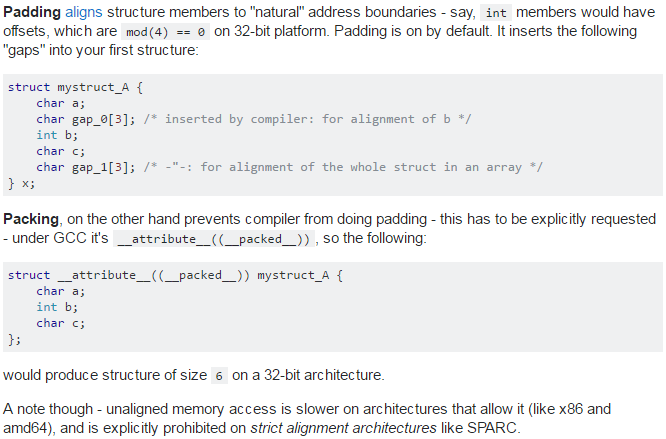
\includegraphics[width=14cm]{packed.PNG}
\end{figure}

\question{8}
\begin{lstlisting}
int global;
void main(void)
{
        int local;
        int *ptr1 = (int *)malloc(sizeof(*ptr1));
        int *ptr2 = (int *)malloc(sizeof(*ptr2));

        printf("global %p loc %p p1 %p p2 %p\n", &global, &local, ptr1, ptr2);
}
\end{lstlisting}
\TODO

\question{9}
\TODO

\question{10}
\ingi{Listes chaînées: concepts de base}{https://inginious.info.ucl.ac.be/course/LSINF1252/linked_lists_1}
\begin{lstlisting}
typedef struct node {
  int value;
  struct node *next;
} node;

size_t length(node *list)
{
    if(list==NULL)
        return 0;

    int count = 1;
    while (list->next != NULL)
    {
        list = list->next;
        count++;
    }

    return count;
}

size_t count(node *list, int value)
{
    if(list == NULL)
        return 0;

    int count = 0;
    while (list !=NULL)
    {
        if(list->value == value) count++;
        list = list->next;
    }
    return count;
}

int push(node **list, int value)
{
    node *n;
    n = (node *)malloc(sizeof(node));
    if(n == NULL)
        return -1;
    n->value = value;
    n->next = *list;
    *list = n;
    return 0;
}

int pop(node **list)
{
    if(list==NULL)
        return 0;

    int r;
    struct node *removed=*list;
    r = (*list)->value;
    *list = (*list)->next;
    free(removed);
    return r;
}

void free_list(node *list)
{
    struct node* tmp;

    while (list != NULL)
    {
        tmp = list;
        list = list->next;
        free(tmp);
    }
}
\end{lstlisting}

%--------------------------------------S4--------------------------------------
\section{Organisation des ordinateurs et étude de cas : IA32} %4
\subsection{QCM}
\TODO
\subsection{Exercices}

%--------------------------------------S5--------------------------------------
\section{Compléments de C et utilisation de plusieurs threads} %5
\subsection{QCM}
\TODO
\subsection{Exercices}

\question{1}
La fonction \manpage{pthread\_join}{3} utilise un deuxième argument de type \lstinline|void**|.
Pourquoi est-il nécessaire d'utiliser un pointeur vers un pointeur et pas simplement un \lstinline|void*| ?

\begin{solution}
Souvent, nos threads vont vouloir retourner un pointeur vers une zone mémoire allouée
sur le tas. C'est pour ça que nos threads retournent \lstinline{void*}.

Du coup, \manpage{pthread\_join}{3} doit recevoir un pointeur vers une variable du même
type que ce qu'on retourne, vu qu'elle va modifier la variable. Ce qu'on retourne
étant un \lstinline{void*}, l'argument de \manpage{pthread\_join}{3} doit être un \lstinline{void**}.
\begin{itemize}
    \item \lstinline{void} ou tout autre type ne servirait à rien : \lstinline{pthread_join} ne
    pourrait pas modifier la moindre variable pour l'utilisateur.
    \item \lstinline{void*} ne permet que de retourner une valeur non-pointeur, et pas un pointeur
    (sauf en faisant un cast, ce qui est très dégueulasse). \lstinline{pthread_join} peut par
    exemple mettre un \lstinline{int}, mais pas un \lstinline{int*}
    \item \lstinline{void**} permet à \lstinline{pthread_join} de modifier l'argument et d'éventuellement y
    mettre un pointeur générique (\lstinline{void*})
\end{itemize}
\end{solution}

\question{2}
À votre avis, pourquoi le premier argument de la fonction \manpage{pthread\_create}{3} est-il un pointeur de type \lstinline|pthread_t*|
alors que le premier argument de la fonction \manpage{pthread\_join}{3} est lui simplement de type \lstinline|pthread_t| ?

\begin{solution}
\manpage{pthread\_create}{3} doit modifier la structure qu'on lui passe en argument (il doit l'initialiser),
tandis que \manpage{pthread\_join}{3} se contente d'accéder aux valeurs qu'on lui passe en argument, et ne les modifie pas.
\end{solution}

\question{3}
Avec les threads POSIX, comment peut-on passer plusieurs arguments à la fonction démarrée par \manpage{pthread\_create}{3} ?
Écrivez un petit exemple en C qui permet de passer un entier et un caractère à cette fonction.

\begin{solution}
La manière la plus simple de le faire est de définir une structure contenant un entier et un caractère, et de passer un pointeur vers cette structure au thread. Par exemple,

\lstinputlisting[linerange={7-33}]{src/ape5q3.c}
\end{solution}

\question{4}
Ecrivez un code qui permet de récupérer un tableau d’entiers d’un thread. Exercice disponible sur \href{https://inginious.info.ucl.ac.be/course/LSINF1252/threads_1}{INGInious}.

\begin{solution}
Faites l'exercice par vous-même ;-).

De manière générale, lorsqu'un thread doit renvoyer une structure de données complexe, ou plusieurs valeurs de retour (tableau statique dont la taille n'est pas connue, liste chainée, tableau et sa taille, plusieurs valeurs de retour), une manière propre de renvoyer ces résultats est de renvoyer une structure spécialement conçue pour retourner toutes ces valeurs. Par exemple, s'il faut renvoyer une liste chainée de mots de passe définie par une \lstinline|struct PasswordList|, ainsi qu'un entier indiquant le nombre total de mots de passe traités (mais pas nécessairement compris dans la liste), on pourrait déclarer une structure
\begin{lstlisting}
struct ThreadReturn {
	int nbrProcessedPasswords;
	struct PasswordList *list;
};
\end{lstlisting}
et le thread retournerait alors un pointeur sur une telle structure : la signature resterait \lstinline|void *my_thread(void *param)| mais les dernières lignes de la fonction seraient
\begin{lstlisting}
struct ThreadReturn *ret = (struct ThreadReturn*) malloc(sizeof(struct ThreadReturn));
if (ret == NULL)
	return NULL;
ret->list = liste; // la liste de mots de passe
ret->nbrProcessedPasswords = nbreMDP; // le nombre de mots de passe lus
return (void*) ret;
\end{lstlisting}
ce qui permet de retourner toutes les valeurs de retour.
\end{solution}

\question{5}
Essayez de lancer un grand nombre de threads d'exécution sur votre machine.
Quel est le nombre maximum de threads que \manpage{pthread\_create}{3} vous autorise à lancer ?

\begin{solution}
Environ $3000$ threads. En tout cas, c'est le maximum de ce qu'il est possible d'avoir sans qu'une segfault plutôt embêtante survient. On peut théoriquement en lancer $100000$ en réduisant la tâche qu'ils doivent accomplir, mais au bout d'un moment les threads lancés au début finissent par se terminer, libérant de la place pour les nouveaux.

Toutes ces valeurs dépendent de l'ordinateur sur lequel les programmes sont utilisés.
\end{solution}

\question{6}
Quelle différence voyez-vous entre \manpage{pthread\_exit}{3} et \manpage{exit}{3} ?

\begin{solution}
\manpage{pthread\_exit}{3} équivaut à un \lstinline|return| dans une des fonctions de thread : ça arrête le thread courant.

\manpage{exit}{3} équivaut à un \lstinline|return| dans la fonction main : ça arrête le programme.
\end{solution}

\question{7}
Un étudiant souhaite passer un tableau d'entiers comme argument à un thread et écrit le code suivant :
\sourcelink{/Programmes/src/}{pthread-array.c}.
Qu'en pensez-vous ?

\begin{solution}
Lors de la fin de l'appel à \lstinline{launch} (qui s'exécute assez rapidement), le tableau \lstinline{v} alloué sur la pile n'est plus accessible, les threads qui s'exécutent reçoivent donc une valeur incorrecte et donc le programme foire (bon, c'est du garbage mais quand même).
\end{solution}

\question{8}
Considérons le programme de test des threads POSIX disponible à l'adresse \sourcelink{/Programmes/src/ }{pthread-test.c}.
Ce programme utilise 4 threads qui incrémentent chacun un million de fois une variable globale.
Exécutez ce programme et observez le résultat qu'il affiche à l'écran. Pouvez-vous expliquer le comportement de ce programme ?

\begin{solution}
De manière assez évidente, on n'atteint jamais $40000000$ mais des trucs intermédiaires : il est fort probable que deux threads exécutent \lstinline|global=increment(global)| en même temps, ce qui a pour conséquence de n'incrémenter \lstinline|global| qu'une fois. Il aurait fallu utiliser des mutex.
\end{solution}

\question{9}
Résolvez des sudokus. Exercice disponible sur INGInious : \url{https://inginious.info.ucl.ac.be/course/LSINF1252/sudoku}

\begin{solution}
Faites l'exercice par vous-même ;-), même s'il n'est pas très intéressant.
%Implémenter un solveur de sudoku en utilisant un algorithme de remplissage aléatoire. Pas très intéressant, mais TODO
\end{solution}


\subsection{Mini-projet : mesure de performance}



% //====================================================\\
% ||                         S6                         ||
% \\====================================================//

\section{Communication entre threads}
\subsection{QCM}
\TODO

\subsection{Exercices}

\question{1}
Écrivez un petit programme qui vous permet de montrer quelles variables sont accessibles à différents threads. Les variables à montrer sont:
\begin{itemize}
	\item variable globale statique
	\item variable globale
	\item variable déclarée dans la fonction main et dont le pointeur est un des arguments aux threads
	\item variable statique déclarée à l’intérieur d’une fonction
	\item variable locale déclarée dans une fonction
\end{itemize}

\begin{solution}
Les variables accessibles aux threads sont :
\begin{itemize}
    \item les variables globales;
    \item les variables dont un pointeur est l'argument d'un des threads;
    \item et les variables globales statiques si la fonction du thread est dans le même fichier (err, \emph{compilation unit}) que cette variable.
\end{itemize}

La variables statique à une fonction n'est accessible que de cette fonction, mais sa valeur est \og commune\fg{} à chaque thread, ce qui fait que ladite fonction n'est \emph{a priori} pas thread-safe.

La variable locale est évidemment accessible qu'à partir de la fonction, et est réinitialisée à chaque appel de la fonction.
\end{solution}

\question{2}
D’après vous (essayez d’expérimenter), que se passe-t-il si:
\begin{itemize}
	\item un thread exécute deux fois \lstinline|pthread_mutex_lock| sur le même mutex d’affilée ?
	\item un thread exécute deux fois d’affilée \lstinline|pthread_mutex_unlock| ?
\end{itemize}

\begin{solution}
Plusieurs fois \manpage{pthread\_mutex\_lock}{3} : il se deadlock lui-même.
Sauf si on a créé un mutex avec gestion des erreurs (\lstinline|PTHREAD_MUTEX_ERRORCHECK|) ; là il détecte le deadlock et renvoie une erreur.

Plusieurs fois \manpage{pthread\_mutex\_unlock}{3} : \emph{undefined behaviour} (en clair, ça crashe, ou alors ça délocke le mutex dans un autre thread, ce qui est rarement voulu).
\end{solution}

\question{3}
Dans la partie théorie, nous avons vu comment s’assurer qu’un seul thread peut accéder à une zone critique à la fois. On vous propose deux solutions (dont une déjà vue dans la partie théorie) :
\begin{lstlisting}
pthread_mutex_lock(&mutex_global);
global=increment(global);
pthread_mutex_unlock(&mutex_global);
\end{lstlisting}
et
\begin{lstlisting}
while (pthread_mutex_trylock(&mutex_global)) ;
global=increment(global);
pthread_mutex_unlock(&mutex_global);
\end{lstlisting}
Discuter les avantages et inconvénients de ces deux solutions (consultez %regardez la man page de
\manpage{pthread\_mutex\_trylock}{3}).

\begin{solution}
Le premier marche (heureusement).

Le deuxième marche \emph{a priori} quand même : on implémente presque le mécanisme interne de \manpage{pthread\_mutex\_lock}{3}.
(La boucle s'arrêtera quand \manpage{pthread\_mutex\_trylock}{3} renverra une valeur nulle, c'est-à-dire quand le mutex a pu être locké.)
%TODO vérifier
\end{solution}

\question{4}
L’outil \lstinline|helgrind| (décrit dans la section helgrind-ref) permet de trouver des deadlocks ou autres problèmes.
Exécutez-le sur le petit programme suivant \sourcelink{/Programmes/src/}{pthread-philo.c}
et analysez ce qu’il affiche.

\begin{solution}
\TODO
% WHAT THE HELL IS GOING ON WITH HELGRIND ??????
\end{solution}



% //====================================================\\
% ||                         S7                         ||
% \\====================================================//

\section{Les sémaphores} %7
\subsection{QCM}
\TODO
\subsection{Exercices}

\question{1}
Expliquez pourquoi la fonction \manpage{sem\_wait}{3} doit prendre comme argument \lstinline|sem_t *|, un pointeur vers une structure \lstinline|sem_t|, et non une structure \lstinline|sem_t|.

\begin{solution}
Pour pouvoir modifier la structure : c'est une file d'attente (contenant les threads en attente) entre autre.
\end{solution}

\question{2}
Dans quels cas la fonction \manpage{sem\_init}{3} risque-t-elle de retourner une erreur ?
\begin{solution}
\begin{itemize}
    \item Le sémaphore est initialisé à une valeur supérieure à la valeur maximale autorisée \lstinline|SEM_VALUE_MAX|.
    \item Le sémaphore a été initialisé pour être partagé entre plusieurs processus, mais l'OS ne supporte pas les sémaphores partagés entre processus.
\end{itemize}
\end{solution}

\question{3}
La librairie POSIX contient également une fonction \manpage{sem\_timedwait}{3}.
Quel intérêt voyez-vous à cette fonction ? Dans quel cas pourrait-elle servir en pratique ?

\begin{solution}
Ce type d'attente est utile dans le cadre de systèmes temps réels.
Dans certains cas, il peut arriver qu'une ressource à laquelle on veut accéder n'ait de sens que jusqu'à un certain moment, et qu'à partir d'un moment, ça ne serve plus rien d'attendre
(typiquement, dans les réseaux, dans les gestions de fichiers, dans les systèmes embarqués ou temps réels).
Dans ce cas, autant indiquer qu'on est près à attendre un certain temps, et passé ce temps ça ne sert plus à rien d'attendre.
Dans le cadre de ce cours, il y a peu d'utilité.
% Même si je connais quelqu'un qui avait proposé cela comme solution pour un producteur-consommateur ;)

Si le temps a été dépassé, la valeur de retour est de -1, et une erreur \lstinline|ETIMEDOUT| est présente.
Si le sémaphore est bloqué au moment de l'appel, et que le temps d'attente est erroné, alors une erreur \lstinline|EINVAL| est présente.
\end{solution}

\question{4}
Un étudiant propose d'implémenter le producteur du problème des producteurs-consommateurs de la façon suivante :
\begin{lstlisting}
// Producteur
void producer(void)
{
	int item;
	while(true)
	{
		item=produce(item);
		pthread_mutex_lock(&mutex);   // modification
		sem_wait(&empty);             // modification
		insert_item();
		pthread_mutex_unlock(&mutex);
		sem_post(&full);
	}
}
\end{lstlisting}
Que pensez-vous de cette solution (en supposant que le consommateur continue à fonctionner comme dans les notes) ?

\begin{solution}
Si lors de l'appel à \lstinline|sem_wait(&empty)|, il n'y a aucune case de libre, alors le thread va bloquer.
Cela peut arriver parce qu'un producteur a rempli la dernière case juste avant, et qu'il est sorti de toutes ses sections critiques.
Le problème, c'est que le seul autre thread qui peut incrémenter \lstinline|empty| est un thread consommateur.
Or, pour qu'un thread consommateur puisse s'exécuter, vider une case du buffer et incrémenter \lstinline|empty|, il doit nécessairement s'approprier le mutex qui a été verrouillé par le producteur.
De même, aucun consommateur n'était en train d'approvisionner le buffer (sinon il posséderait le mutex), et aucun consommateur n'est en train d'exécuter \lstinline|sem_post(&empty)| (ça ne peut arriver que lorsqu'un thread possède le mutex).
On a donc une impossibilité pour le producteur de continuer : deadlock.
\end{solution}

\question{5}
Un autre étudiant propose d'implémenter le consommateur du problème des producteurs-consom\-mateurs comme ceci :%FIXME pas sûr de la position de la coupure
\begin{lstlisting}
// Consommateur
void consumer(void)
{
	int item;
	while(true)
	{
		sem_wait(&full);
		pthread_mutex_lock(&mutex);
		item=remove(item);
		sem_post(&empty);             // modification
		pthread_mutex_unlock(&mutex); // modification
	}
}
\end{lstlisting}
Que pensez-vous de la solution (en supposant que le producteur n'a pas été modifié) ?

\begin{solution}
L'ordre dans lequel on libère les ressources importe peu : de toute façon, si un thread est bloqué sur les deux ressources, il devra attendre dans tous les cas l'autre avant de pouvoir s'exécuter. Et s'il attend sur une seule, c'est qu'il y a un bug.

Plus précisément, si une interruption a lieu avant \lstinline|sem_post(&empty)|, rien ne change.
Si une interruption a lieu après \lstinline|pthread_mutex_unlock(&mutex)|, rien ne change non plus.
Si une interruption a lieu entre les deux (le cas où une interruption survient pendant les appels est implicitement géré par les fonctions appelées),alors on se retrouve avec l'indication d'une nouvelle case libre dans le buffer, mais avec un buffer toujours inaccessible.
Si un thread était bloqué sur un \lstinline|sem_wait(&empty)|, il va peut-être être débloqué, mais il sera arrêté par son appel à \lstinline|pthread_mutex_lock(&mutex)| : le buffer n'a pas encore été libéré.
Si aucun thread n'était bloqué sur \lstinline|sem_wait(&empty)|, ils sont de toutes façons déjà bloqués sur le mutex.
Donc, les autres threads doivent quand même attendre \manpage{pthread\_mutex\_unlock}{3} pour pouvoir enfin s'exécuter, et il n'y a donc pas plus de violation de section critique.
Et comme ce sont deux appels non bloquant, aucun risque d'avoir un deadlock.
\end{solution}

\question{6}
Un étudiant propose de résoudre le problème du rendez-vous en utilisant le code ci-dessous. Comparez sa solution avec celle vue au cours.

\begin{solution}
\TODO
% Ce qui suit est une spéculation de réponse ; j'avais l'impression que ça ne marchait pas, puis en écrivant je me suis rendu compte qu'il était bien probable que ça marche, et finalement j'ai vu que ça marchait.

%Supposons qu'il ne reste plus que deux threads avant que la barrière soit levée. Il est bien probable qu'une interruption ait lieu entre le \lstinline|pthread_mutex_unlock(&mutex)| et le moment où le \lstinline|if| et sa condition s'exécutent. Entre temps, vu que le mutex aura été changé, peut-être qu'un autre thread va venir modifier la valeur de \lstinline|count|, qu'il sortira lui aussi de sa section critique, et qu'il sera lui aussi interrompu avant le \lstinline|if|. Dans ce cas, si le premier thread revient à la charge, il verra que count vaut le nombre de thread requis, et va donc libérer les autres threads via sem_post, qui passeront ainsi le rendez-vous. Néanmoins, il restera un autre thread qui lui n'aura pas encore complètement fini. Mais il ne pourra faire qu'une seule chose : un sem_post supplémentaire, qui n'aura aucune influence sur le reste du déroulé du programme vu que tous les threads auront atteint la barrière quand cet espèce de foutoir aura lieu. En pratique, cette solution marche également, même si elle est moins clean que l'autre, et qu'elle peut faire plus de sem_post que nécessaire.

%TODO : je ne suis pas sûr, mais j'ai l'impression qu'en fait ça marche quand même
\end{solution}

\question{7}
Considérons un problème du rendez-vous avec 13 threads. Lorsque tous les threads ont passé le rendez-vous, quelle sera la valeur du sémaphore \lstinline|rendezvous| renvoyée par la fonction \manpage{sem\_getvalue}{3} ?

\begin{solution}
Avec $N$ threads, il y a exactement $N$ appels à \manpage{sem\_wait}{3} qui décrémente la valeur du sémaphore, et $N+1$ appels à \manpage{sem\_post}{3} qui incrémentent la valeur du sémaphore.
Comme le sémaphore est initialisé à $0$ (pour que le premier thread arrivant soit déjà bloqué), à la sortie de la barrière, il aura la valeur $1$ ($0+(N+1)-N = 1$).
Et normalement, tant qu'on implémente bien une égalité stricte, ça marche.
\end{solution}

\question{8}
La librairie POSIX contient la fonction \manpage{sem\_getvalue}{3} qui permet de récupérer la valeur d’un sémaphore sans pour autant effectuer d’opération \manpage{sem\_wait}{3} sur ce sémaphore.
Elle peut être utilisée pour observer l’évolution de la valeur d’un sémaphore.
Modifiez le programme des philosophes contenant un deadlock (\sourcelink{/Programmes/src/}{pthread-philo-sem.c})
et ajoutez-y un thread qui observe toutes les 10 secondes l’évolution des sémaphores et arrête tout le programme via \manpage{exit}{3} en affichant un message d’erreur si les valeurs des sémaphores n’ont pas changé.

\begin{solution}
Le code suivant effectue cela. La variable \lstinline|busy| indique que le programme est actif ; il est mis à 1 au début du programme (dans la \lstinline|main|) et passe à 0 juste avant la fin.
\begin{lstlisting}
void *spectateur(void *arg)
{
	int past_valeurs[PHILOSOPHES];
	memset(past_valeurs, -1, sizeof(past_valeurs));
	while (busy) {
		int changed=0;
		for (long i=0; i<PHILOSOPHES; i++) {
			int curvalue;
			int err = sem_getvalue(&baguette[i], &curvalue);
			if (err!=0)
				exit(EXIT_FAILURE);
			if (curvalue != past_valeurs[i])
				changed=1;
			printf("Baguette %d : %d (avant %d) (utilisée par philosophes %d et %d)\n", (int)i, curvalue, past_valeurs[i], (int)i, (int)(i-1)%PHILOSOPHES);
			past_valeurs[i] = curvalue;
			}
		if (!changed) {
			printf("No value changed since 10s ago - killing myself\n");
			fflush(stdout);
			exit(EXIT_FAILURE);
		}
		usleep(10*1000*1000);
	}
	return NULL;
}
\end{lstlisting}
\end{solution}

\question{9}
Les mutex et les sémaphores peuvent être utilisés pour résoudre des problèmes d’exclusion mutuelle.
Le programme \sourcelink{/QCM/S7/src/}{pthread-mutex-perf.c} utilise des mutex.
Modifiez-le pour utiliser des sémaphores à la place et comparez le coût en termes de performance entre les mutex et les sémaphores.

\begin{solution}
Voir codes fournis.

Étrangement, dans les cas où la section critique est relativement courte ($<60$), cela prend plus de temps d'utiliser des mutex que d'utiliser des sémaphores. Un peu contre-intuitif.
\end{solution}



% //====================================================\\
% ||                         S8                         ||
% \\====================================================//

\section{Les processus}
\subsection{QCM}
\TODO
\subsection{Exercices}
\question{1}
Dans quels cas l'appel système \manpage{fork}{2} peut-il retourner une erreur ? Pourriez-vous construire un petit programme dans lequel \manpage{fork}{2} retourne une erreur ?

\begin{solution}
La majorité des erreurs viennent de limitations mémoire :
\begin{itemize}
    \item pas assez de mémoire pour allouer les \og \emph{necessary kernel structure}\fg{} ;
    \item pas réussi à allouer assez de mémoire pour tout copier.
\end{itemize}

Un dernier cas est possible : on a atteint la limite supérieure au nombre total de processus pouvant être créés sur l'ordinateur (\#forkbomb).

Le plus simple pour provoquer une erreur est de créer un programme qui crée un nombre invraisemblable de processus, afin de saturer l'ordinateur. On peut par exemple utiliser le programme du QCM.
\end{solution}

\question{2}
Dans quels cas l'appel système \manpage{wait}{2} peut-il retourner une erreur ?
Pourriez-vous écrire un programme dans lequel \manpage{wait}{2} retourne une erreur ?

\begin{solution}
Généralement, c'est parce que la fonction a été mal appelée :
\begin{itemize}
    \item pas de processus avec cet identifiant, ou alors quelqu'un l'attend déjà ;
    \item mauvais arguments ;
    \item un signal SIGCHLD (indiquant le décès d'un fils\footnote{Repose en paix petit ange ;-)})
    a été reçu alors qu'on avait explicitement demandé à ne pas devoir en gérer ;
    \item il n'y a plus de processus fils.
\end{itemize}
On peut donc faire planter \manpage{wait}{2} en l'appelant deux fois sur le même identifiant de processus, ou en demandant au système d'enterrer immédiatement les processus fils.
\end{solution}

\question{3}
L’appel système \manpage{fork}{2} retourne l’identifiant du processus fils dans le processus père.
Imaginez qu’une variante de Unix choisisse d’implémenter \manpage{fork}{2} en retournant 0 dans le processus fils et 1 dans le processus père.
Quel serait l’impact de cette modification pour un programme qui lance plusieurs processus fils ?

\begin{solution}
Le processus père ne pourrait plus retrouver ses enfants.
\end{solution}

\question{4}
Combien de processus sont créés lors de l'exécution du (morceau de) programme suivant ?
\begin{lstlisting}
// ...
fork();
fork();
// ...
\end{lstlisting}

\begin{solution}
On note $P$ le processus père, puis $A_1$ son fils de degré 1, $A_2$ le fils du fils, $B_1$ le second fils du père.
\begin{enumerate}
    \item Avant le premier fork : juste $P$
    \item Après le premier fork et avant le second fork : $P$ ainsi que $A_1$.
    \item Après le premier fork et avant le second fork : $P$ ainsi que $A_1$.
    \item Après le deuxième fork dans le processus fils : $A_1$ ainsi que $A_2$, et $P$ et ses enfants en arrière plan. Il ne va plus en créer, ses enfants non plus.
\end{enumerate}

On a donc 4 processus : $P$, $A_1$, $A_2$ et $B_1$.
\end{solution}

\question{5}
En supposant que le processus père a comme identifiant la valeur 1252, représentez graphiquement sous forme d’un arbre l’ensemble des processus créés par le programme ci-dessus en supposant que les identifiants de processus sont attribués séquentiellement par le kernel.
\begin{solution}
% Flemme de faire autre chose que de l'ASCII art
\begin{lstlisting}
               Père P
                1252
               /     \
              /       \
       Fils A1        Fils B1
        1253       1255 ou 1254(*)
       /
      /
    Fils A2
1254 ou 1255(*)
\end{lstlisting}

(*) : ça dépend de si le père ou le fils s'exécute en premier après le premier appel à \manpage{fork}{2}. Si le père commence (continue) avant le fils, B1 aura un pid de 1254 et A2 de 1255 ; si c'est le fils qui commence, $A_2$ aura le pid de 1254 et $B_1$ aura 1255.
\end{solution}

\question{6}
L’appel système \manpage{fork}{2} est nécessaire au fonctionnement de Unix.
Cependant, un programme qui abuse de \manpage{fork}{2} risque de perturber le fonctionnement du système.
Que risque-t-il d’arriver si vous exécutez un programme qui par mégarde contient :
\begin{lstlisting}
while(true) {
	fork();
	// ...
}
\end{lstlisting}
Consultez les pages de manuel pour déterminer comment le système d'exploitation
peut se protéger contre de telles \href{http://en.wikipedia.org/wiki/Fork_bomb}{fork bomb}

\begin{solution}
Il va constituer une \emph{fork bomb} : des milliers de processus vont être créés, et ça va ralentir le système (vu qu'il doit, par principe, laisser chaque processus s'exécuter) et prendre beaucoup de ressources au niveau CPU et mémoire.
Pour éviter ça, le kernel se protège des utilisateurs en instaurant une limite au nombre maximum de processus (généralement par utilisateur) pouvant tourner en même temps sur un ordinateur.
Si le maximum est atteint, plus aucun nouveau processus ne peut être créé.
Par défaut, Linux ne copie pas immédiatement un processus et sa mémoire, mais ne copie que lorsqu'on modifie la mémoire (\emph{copy on write}) ;
du coup, ça ralentit les accidents mais c'est quand même dangereux.
\end{solution}

\question{7}
Comparez les performances de la création et la terminaison de threads et de processus
en compilant et exécutant sur un ordinateur non chargé les programmes
\sourcelink{/Programmes/src/ }{fork-perf.c} et
\sourcelink{/Programmes/src/ }{pthread-perf.c}.
Utilisez la commande \manpage[posix]{time}{1} pour mesurer le temps d’exécution de chacun des ces programmes qui créent 100000 processus ou threads.
Expliquez vos résultats.

\begin{solution}
Assez évidemment, le programme avec les processus prend bien plus de temps que le programme avec les threads.
\end{solution}

\question{8}
Compilez le programme
\sourcelink{/Programmes/src/}{fork-zombie.c}.
Ce programme crée un processus mais le processus père attend une minute pour récupérer sa valeur de retour.
Lancez ce programme en tâche de fond (voir section outils) et utilisez \manpage{ps}{1} ou consultez le dossier \filepath{/proc/}.

\begin{solution}
\manpage{ps}{1} indique qu'un processus est \og defunct \fg{} (il s'est terminé, et est un zombie).
\manpage{top}{1} est plus explicite : il y a vraiment un zombie.
\end{solution}

\question{9}
La librairie standard comprend une fonction \manpage{system}{3} qui permet l’exécution d’une commande du shell.
Ainsi, la ligne \lstinline|system("for f in {1..3} ; do echo $f ; done");| va provoquer un appel au shell bash
qui va exécuter la commande passé en argument et donc afficher trois lignes contenant chacune un nombre sur la sortie standard.
Quels sont les appels systèmes utilisées par une implémentation de cette fonction \manpage{system}{3} ?

\begin{solution}
Note : \manpage{system}{3} est fortement déconseillé par le manuel lorsque le processus appelant a des privilèges au-dessus de la moyenne.

Autre note : il vaut mieux utiliser \cmdline{/usr/bin/echo} au lieu de \cmdline{echo} ;
echo est une commande de bash, et il ne crée donc pas de processus.
De même, il est fort probable que le shell appelé par \manpage{system}{3} ne puisse pas exécuter la commande convenablement ;
il faut alors directement utiliser \manpage{execve}{2} et ses dérivés.

Une commande particulièrement utile pour examiner les appels systèmes effectués est \manpage{strace}{1} ;
en rajoutant l'option \lstinline|-f|, on peut également examiner les appels systèmes des processus enfants.

Au tout début, on a un appel à \manpage{execve}{2} qui permet de lancer le processus.

Début de la fonction, pleins de boilerplate, notamment pour charger toutes les bibliothèques partagées, allouer suffisamment de mémoire, protections de zones mémoire, etc.

\lstinline|fork()| pour créer un processus fils.

Dans le père : \manpage{waitpid}{2} du processus fils.
Quand il l'a reçu, quelques clean-up et retourne.

Dans le fils :
On ne redirige pas les flux d'erreurs.
On appelle \lstinline|execve("/bin/bash", {"bash", "for f in {1..3} ; do echo $f ; done", NULL}, NULL)|.
Le processus nouvellement créé va alors exécuter la commande, et va donc à 3 reprises exécuter \lstinline|echo|, donc
\begin{itemize}
	\item \manpage{fork}{2} et \manpage{waitpid}{2} (ou plutôt \manpage{wait4}{2})
	\item redirection des entrées-sorties
	\item \lstinline|execve("/bin/echo", {"echo", f, NULL}, NULL)|
\end{itemize}
Et va finalement retourner.

Sachant qu'à chaque fois qu'on affiche quelque chose, il y a des \manpage{read}{2} et \manpage{write}{2} qui surviennent,
on constate qu'il y a quelques appels systèmes qui surviennent. Oh, pas beaucoup : deux centaines.
% FIXME je ne parviens plus à vérifier cette réponse avec mon programme ; il est donc possible que ce soit faux.

\end{solution}

\question{10}
Quelles différences et similitudes voyez-vous entre
\begin{itemize}
	\item \manpage{pthread\_create}{3} et \manpage{fork}{2} ?
	\item \manpage{pthread\_join}{3} et \manpage{waitpid}{2} ?
\end{itemize}

\begin{solution}
\manpage{pthread\_create}{3} et \manpage{fork}{2} : permettent tous deux de créer un nouveau thread/processus.

Différence : \manpage{pthread\_create}{3} nécessite que l'on spécifie la fonction principale du thread,
tandis que \manpage{fork}{2} se sert de la fonction actuelle.

A vrai dire, sous Linux, \manpage{pthread\_create}{3} et \manpage{fork}{2} appelle l'appel système \manpage{clone}{2}, qui se débrouille pour émuler les deux systèmes.

\manpage{pthread\_join}{3} et \manpage{waitpid}{2} : permettent tous deux d'attendre la fin d'un thread/processus.

Très peu de différences au final d'ailleurs !
\end{solution}

\question{11}
La commande \manpage{strace}{1} permet de tracer tous les appels systèmes faits par un programme.
Recompilez un programme d’exemple et essayer d’identifier les principaux appels systèmes qui sont utilisés par ce programme.
Les paramètres \lstinline|-c|, \lstinline|-t| et \lstinline|-e|
peuvent être utiles pour explorer le comportement d’un programme et avoir une idée des appels systèmes qu’il effectue.

\nosolution{}
\TODO

\question{12}
La commande \manpage{pstree}{1} permet de visualiser sous forme d’arbre l’ensemble des processus actifs sur un ordinateur Linux.
Exécutez \manpage{pstree}{1} et identifiez quels sont les processus qui sont les ancêtres de votre commande.

\begin{solution}
Tous les processus descendent de \lstinline|systemd| (oh non\dots diront certains), et on voit bien tous les processus.

Petite subtilité : quand un processus est lancé deux fois, il n'apparait qu'une fois mais avec un petit 2 à côté. Autre subtilité : entre accolades ($\{ \}$), on a le nombre de threads enfants du processus.
\end{solution}

\question{13}
Un shell tel que \manpage{bash}{1} permet à l’utilisateur de lancer plusieurs programmes simultanément.
Par exemple, il est possible de lancer un programme en \emph{background} (ou tâche de fond en français) en le suffixant avec le caractère \&.
On peut faire de même en tapant Ctrl-Z (les touches Ctrl et Z simultanément) pendant qu’un programme s’exécute.
Cela peut être utile pour taper une commande pour par exemple voir l’état du système pendant l’exécution du programme.
Il est possible de revenir à l’exécution du programme via la commande \manpage[posix]{fg}{1}.
La commande \manpage[posix]{jobs}{1} permet de lister les processus qui sont actuellement exécutés par le shell en tâche de fond.
La section \emph{JOB CONTROL} du manuel de \manpage{bash}{1} fournit plus d’informations à ce sujet.

\begin{solution}
Merci la documentation ;-)
\end{solution}

\question{14}
Le répertoire \filepath{/proc} contient une image de la table des processus maintenue par le kernel et d’autres structures de données maintenues par le kernel.
Compilez le programme
\sourcelink{/Programmes/src/}{fork-pthread.c}
qui lance un processus fils puis crée un thread à l’intérieur du processus père.
Lancez ce programme en background via \cmdline{bash} et observez les entrées relatives au père, au fils et au thread créé par le processus père dans \filepath{/proc/}.

\begin{solution}
On voit bien le \emph{process id}, le \emph{parent process id} et le nombre de thread du processus père.
On voit aussi qu'ils sont tous attachés au processus bash.
\end{solution}



% //====================================================\\
% ||                         S9                         ||
% \\====================================================//

\section{Utilisation du système de fichiers et les \textit{pipe}}
\subsection{QCM}

\subsection{Exercices}

\question{1}
Consultez la page de manuel de \manpage{chmod}{1} ou d’autres sources pour déterminer
la signification des bits de permissions lorsqu'ils sont associés à un répertoire.
Expliquez notamment à quoi sert le bit d’exécution sur un répertoire.

\begin{solution}
\begin{itemize}
\item r : est-il possible d'afficher le contenu du répertoire ?

\item w : est-il possible de renommer, créer ou supprimer un fichier dans ce répertoire, ou de modifier les attributs du répertoire ?

\item x : est-il possible d'ouvrir ce répertoire ?
Avec \manpage{chmod}{1}, il y a aussi le \og bit\fg{} X qui permet de ne viser que ce bit de permission sur les répertoires.
Par exemple, \cmdline{chmod -R u-x, u+X}

\item s : \emph{Set User ID} ou \emph{Set Group ID} : en remplacement du bit d'exécution de l'utilisateur ou du groupe.
Lors de la création d'un fichier par un utilisateur 1, celui-ci aura comme propriétaire le propriétaire du dossier (utilisateur 2), et non celui du créateur, 1.
Lors de la création d'un sous-dossier, celui-ci héritera de cette permission, et de ce propriétaire.
C'est un peu compliqué, et c'est expliqué extrêmement mal dans le manuel (comprendre : c'est complet mais illisible) ;
je vous encourage à recherche sur Google et Wikipedia de plus amples informations.

\item t : est-ce que les fichiers et dossiers contenus à l'intérieur peuvent être supprimés ou renommés par les autres utilisateurs que ceux du groupe ou du propriétaire (ex : \filepath{/tmp/}).
S'il y est, ce n'est pas le cas.
\end{itemize}
\end{solution}

\question{2}
Quelles sont les permissions associées à votre répertoire de login ?
Ces permissions permettent-elles à d’autres étudiants d’accéder à vos fichiers ?
Si oui, utilisez \manpage{chmod}{1} pour supprimer cette autorisation de lecture par défaut dans votre répertoire.

\begin{solution}
Désormais, $700$ : je peux y entrer, mais personne d'autre. Logique en fait.
\footnote{On se souviendra du seul utilisateur de 2017 qui avait ses bits de permissions à $744$.}
\end{solution}

\question{3}
Comment feriez-vous en utilisant \manpage{chmod}{1} pour créer un répertoire dans lequel vous pouvez lire et écrire, tout étudiant peut lire mais aucun membre du staff (à part l’administrateur système bien entendu) ne peut lire ?

\begin{solution}
\begin{lstlisting}
mkdir folder % 755
chmod 640 folder
\end{lstlisting}
\end{solution}

\question{4}
Le répertoire \filepath{/tmp/} est particulier car il est destiné à pouvoir contenir des fichiers de n’importe quel utilisateur.
Pouvez-vous expliquer les permissions utilisées pour ce répertoire ?

\begin{solution}
Le 't' indique que le répertoire n'autorise pas les autres utilisateurs à supprimer ou renommer des fichiers ou des dossiers d'un utilisateur.
Pratique pour éviter de voir son travail perdu.
\end{solution}

\question{5}
La commande \manpage{lsof}{8} permet de lister les fichiers ouverts par un processus.
A votre avis, comment cette commande fonctionne-t-elle ?

\begin{solution}
Elle regarde dans le dossier spécial \filepath{/proc/[pid]/fd} pour chaque processus, la liste des \emph{file descriptors} et donc des fichiers ouverts.
\end{solution}

\question{6}
Lorsqu’un exécutable est lancé avec \manpage{execve}{2}, il hérite des descripteurs de fichiers qui étaient ouverts dans le processus qui a exécuté \manpage{execve}{2}.
Comment feriez-vous en utilisant uniquement l’appel système \manpage{open}{2} pour déterminer combien de descripteurs de fichiers étaient ouverts au démarrage de votre programme ?

\begin{solution}
Comme les descripteurs de fichier sont attribués séquentiellement, on peut appeler \manpage{open}{2}, récupérer sa valeur de retour et soustraire $1$.
En particulier, sachant que $0$, $1$ et $2$ sont associés à l'entrée standard, la sortie standard et la sortie d'erreurs standard, recevoir comme valeur de retour 3 indique qu'aucun fichier n'a précédemment été ouvert.

(C'est la réponse officielle des tuteurs ;
évidemment, si le processus parent s'est amusé à ouvrir pleins de fichiers puis à fermer le premier fichier ouvert,
\manpage{open}{2} renverra quand même l'ancien descripteur de ce fichier, alors qu'il reste d'autres fichiers ouverts.
Parfois, les réponses ne sont pas correcte.)
\end{solution}

\question{7}
Est-il possible dans un processus d’exécuter \lstinline|int fd1 = open("f",O_RDWR)| ;
et juste après \lstinline|int fd2 = open("f",O_RDONLY);| ?
Si oui, quelles seront les valeurs des descripteurs de fichiers retournés lors des appels système.
Si non, quelles seront les valeurs de \lstinline|errno| ?

\begin{solution}
C'est parfaitement possible.
En pratique, le premier \emph{file descriptor} référera à un \emph{open file object} sur lequel on peut lire et écrire,
et le deuxième \emph{file descriptor} référera à un autre \emph{open file object}, avec ses propres propriétés et son propre \emph{file offset}, sur lequel on ne pourra que lire.
Les deux descripteurs de fichier seront évidemment différents.
\end{solution}

\question{8}
Dans un shell, on exécute la commande \cmdline{/bin/echo "1234" > ./test.txt}.
Quels sont les appels systèmes effectués par le shell avant l’exécution de \cmdline{/bin/echo} ?

\begin{solution}
Déjà, le shell se fork.

Dans le fils, on ferme le \emph{file descriptor} correspondant à \lstinline|stdout|, on ouvre le fichier \filepath{test.txt}
(logiquement, le \emph{file descriptor} renvoyé sera $1$, correspondant à la sortie standard).

(Alternative : ouvrir le fichier 'test.txt' dans un \emph{file descriptor} \lstinline|fdtest|,
puis dupliquer avec \manpage{dup2}{2} : \lstinline|dup2(fdtest, STDOUT_FILENO)|
(\lstinline|STDOUT_FILENO| est d'abord fermé, puis devient une copie de \lstinline|fdtest|)
(\manpage{dup2}{2} renvoie \lstinline|STDOUT_FILENO| comme nouveau \emph{file descriptor}, ou $-1$ s'il y a une erreur).)

Enfin, appel à \manpage{execve}{2} : le processus va alors croire qu'il écrit sur le terminal, dans \lstinline|stdout|, alors qu'il écrit dans un fichier.
\end{solution}

\question{9}
Dans un shell, on exécute la commande \cmdline{./a.out < in.txt > out.txt}.
Quelles sont les appels systèmes qui doivent être exécutés par le shell pour lancer cet exécutable comme demandé par l’utilisateur ?

\begin{solution}
Similaire à la Q8 :
\begin{lstlisting}
int pid = fork();
if (pid < 0)
exit(EXIT_FAILURE);
else if (pid == 0) {
	// fils
	if (close(STDIN_FILENO))
	_exit(EXIT_FAILURE);
	int fdin = open("in.txt", O_RDONLY | O_CREAT, S_IRUSR | S_IWUSR); // logiquement, c'est 0
	if (fdin == -1)
	_exit(EXIT_FAILURE);
	if (close(STDOUT_FILENO))
	_exit(EXIT_FAILURE);
	int fdout = open("out.txt", O_WRONLY | O_CREAT | O_TRUNC, S_IRUSR | S_IWUSR); // logiquement, c'est 1
	if (fdout == -1)
	_exit(EXIT_FAILURE);
	execve("a.out", {"a.out", NULL}, NULL);
	_exit(EXIT_FAILURE); // normalement, on n'arrive jamais ici
} else {
	int status = 0;
	waitpid(pid, &status, 0);
}
\end{lstlisting}
\end{solution}

\question{10}
Dans un shell, on exécute la commande \cmdline{cat < in.txt | grep sinf1252}.
Quelles sont les appels systèmes qui doivent être exécutés par le shell pour lancer cette commande comme demandé par l’utilisateur ?

\begin{solution}
\begin{lstlisting}
fork(); // pour créer le processus qui va effectuer grep
\end{lstlisting}
dans le père :
\begin{lstlisting}
waitpid(fils); // on attend donc celui qui va faire grep.
\end{lstlisting}

Dans le fils :
\begin{lstlisting}
int fd1[2];
pipe(fd1); // crée le pipe entre les deux processus
fork()
\end{lstlisting}

Dans le fils du fils :
\begin{lstlisting}
close(fd1[0]); // fermer le côté lecture, vu qu'on va écrire
close(STDIN_FILENO)
int fdin1 = open("in.txt", O_RDONLY | O_CREAT); // vu que STDIN_FILENO a été fermé, ça vaut désormais 0, l'entrée standard.
int fdout1 = dup2(fd1[1], STDOUT_FILENO); // ferme STDOUT_FILENO dans ce processus, et le remplace par le côté écriture du pipe.
execve("/bin/cat", {"cat", NULL}, NULL); // appel à cat, même si tout ce qu'il va faire c'est piper l'entrée standard à la sortie standard.
\end{lstlisting}

Dans le père du fils (l'ancien fils, en fait) : (dernier à s'exécuter)
\begin{lstlisting}
close(fd1[1]); // fermer le côté écriture, vu qu'on va lire
// STDOUT_FILENO reste ouvert, et c'est le nôtre.
int fdin2 = dup2(fd1[0], STDIN_FILENO); // ferme STDIN_FILENO dans ce processus, et le remplace par le côté lecture du pipe.
execve("/usr/bin/grep", {"grep", "lsinf1252", NULL}, NULL);
\end{lstlisting}
\end{solution}

\question{11}
Dans un shel \manpage{bash}{1}, lorsque l’on suffixe une commande avec \cmdline{2>\&1},
le shell redirige la sortie d’erreur standard vers la sortie standard.
Quels sont les appels systèmes utilisés par le shell pour réussir cette redirection ?

\begin{solution}
Syntaxe : \cmdline{commande > out.txt 2>&1} ou \cmdline{commande 2>&1 | grep}
si l'on veut afficher tout le contenu sur la sortie standard, par exemple pour chainer.

\begin{lstlisting}
fork();
int fdout("out.txt", O_WRONLY | O_CREAT | O_TRUNC, ...); // version avec redirection dans un fichier.
int fdout1 = dup2(fdout, STDOUT_FILENO);
int fderr1 = dup2(fdout, STDERR_FILENO);
execve("commande", {NULL}, NULL);
\end{lstlisting}
\end{solution}

\question{12}
Comment se comporte l’appel système \manpage{write}{2} lorsque le disque sur lequel on souhaite écrire des données est plein ?
Peut-on distinguer cette erreur d’un problème d’écriture sur le disque ?

\begin{solution}
L'appel échoue avec le code d'erreur \lstinline|ENOSPC| dans \lstinline|errno|.
\end{solution}

\question{13}
A quoi sert l’appel système \manpage{sync}{2} ?

\begin{solution}
sync force l'écriture sur disque de toutes les données présentes dans les buffer du système d'exploitation.

Très utile quand on utilise des clés USB ou autre, qui peuvent être débranchées inopinément.

Néanmoins, rien ne garantit que les données ont bien été écrites sur le support de stockage, si celui-ci a un grand cache de donnée et reporte que tout va bien.
\end{solution}

\question{14}
Le programme \sourcelink{/Programmes/src/}{writeperf.c}
permet de tester les performances des écritures dans \manpage{write}{2} sur un système de fichiers.
Compilez-le et exécutez le avec différents tailles de buffers passés à \manpage{write}{2}.
Mesurez le temps d’exécution avec la commande \manpage[posix]{time}{1} et comparez le temps qu’il faut pour écrire 100MB en blocs de 1 MB ou en blocs de 1 KB.
Faites de même en activant la synchronisation avec le paramètre \cmdline{-s}.

\begin{solution}
De manière assez logique, plus on réduit la taille du buffer, plus il y a d'appels systèmes et plus le processus met du temps à écrire.

Activer sync force l'écriture sur disque, et bypasse le buffer du système d'exploitation : ça ralentit encore plus pour des petits blocs de données.
\end{solution}



% //====================================================\\
% ||                         S10                        ||
% \\====================================================//

\section{Les signaux, les sémaphores nommés et le partage de fichiers}

Cette séance d'APE a été effectuée pendant l'année 2016--2017 en S12 au lieu de S10.
Le contenu de cette APE se réfère à la semaine 10 sur le site des exercices.

\subsection{QCM}
\TODO

\subsection{Exercices}

\question{1}
En utilisant \manpage{signal}{2}, écrivez une fonction C \lstinline|sig_ignored| qui prend comme argument un numéro de signal et retourne \lstinline|true| si le signal passé en argument est ignoré par le processus et \lstinline|false| sinon.

\begin{solution}
Le code suivant effectue cette tâche :
\begin{lstlisting}
typedef void (*sighandler_t)(int); // écrire en début de fichier pour permettre d'utiliser le type de donnée sighandler_t

bool sig_ignored(int signum)
{
	sighandler_t ret = signal(signum, SIG_DFL);
	if (ret == SIG_ERR)
		exit(EXIT_FAILURE);
	// ret contient l'ancien signal handler. Du coup, on le remet. Soit ça reste SIG_DFL, soit ça restore
	sighandler_t ret2 = signal(signum, ret);
	if (ret2 == SIG_ERR)
		exit(EXIT_FAILURE);
	return ret == SIG_IGN; // est-ce qu'on avait SIG_IGN avant ?
}

\end{lstlisting}

L'appel signal renvoie l'ancien handler.
On peut donc se permettre de temporairement remplacer le handler actuel par \lstinline|SIG_DFL| avec \manpage{signal}{2}
(pas \lstinline|SIG_IGN| car ça a des conséquences fâcheuses),
récupérer le handler actuel (enfin, l'ancien, mais en fait c'est celui que l'on recherche),
prier pour qu'il n'y ait aucun traitement de signal pendant ce temps là,
puis de nouveau appeler \manpage{signal}{2} pour remplacer le \lstinline|SIG_DFL| par l'\og ancien\fg{} handler (en vrai, celui de départ),
et donc vérifier que ce qu'on reçoit soit bien \lstinline|SIG_DFL|.
On peut alors comparer le handler de départ à \lstinline|SIG_IGN|.

Note au niveau des signaux : par défaut, très peu de signaux sont ignorés (voire même aucun) :
ils apparaissent tous comme étant \lstinline|SIG_DFL|, même ceux qui ont le comportement \lstinline|SIG_IGN|.
La fonction va donc uniquement retourner les signaux ayant changé le handler vers l'ignorage (ou l'ignoration).

Autre petit soucis, affecter \lstinline|SIG_IGN| à un signal dont le comportement par défaut est similaire à \lstinline|SIG_IGN| n'est pas équivalent à lui affecter \lstinline|SIG_DFL|, et l'inverse est aussi vrai.
En effet, ces signaux ne sont pas vraiment \og ignorés \fg{} : c'est le système d'exploitation qui gère leur comportement,
et c'est lorsqu'on demande de changer de comportement que le signal devient ignoré.
Par exemple, SIGCHLD va par défaut être ignoré (au sens, pas de crash ou d'appel de fonction ou de blocage),
et les enfants qui se terminent sans être attendus deviennent automatiquement des zombies.
Si maintenant on ignore explicitement le signal, alors dans ce cas, les processus fils se termineront immédiatement, et il ne sera plus possible de les attendre (vu qu'ils seront morts) ;
pire, il n'est même plus possible d'attendre ses enfants, car ils se terminent directement, et \manpage{waitpid}{2} échoue avec un code d'erreur \lstinline|ECHILD|.
\end{solution}

\question{2}
A votre avis, pourquoi le système d’exploitation refuse-t-il l’exécution de la ligne \lstinline|signal(SIGKILL,SIG_IGN)| ?

\begin{solution}
Le signal SIGKILL ne peut pas être ignoré par le processus ; il le tue obligatoirement.
\end{solution}

\question{3}
Sachant qu’en tapant Ctrl-C durant l’exécution d’un processus le shell envoie un signal SIGINT à ce processus,
comment feriez-vous pour qu’un de vos programmes puisse survivre à Ctrl-C ?

\begin{solution}
On définit un signal handler pour SIGINT, du type :
\begin{lstlisting}
sighandler_t err = signal(SIGINT, survivre);
if (err == SIGERR)
	perror("signal"), exit(EXIT_FAILURE);
\end{lstlisting}
avec
\begin{lstlisting}
void survivre(int signum, sighandler_t handler) {
	// vide
}
\end{lstlisting}
Dans ce cas, le signal va être complètement désactivé.
Point négatif, il est fort probable qu'un SIGKILL s'ensuive par impatience de l'utilisateur\dots

Autre possibilité :
\begin{lstlisting}
sihandler_t err = signal(SIGINT, SIG_IGN);
\end{lstlisting}
\end{solution}

\question{4}
\begin{sloppypar}
Le programme \sourcelink{/Programmes/src/}{alarm.c}
que nous avons utilisé pour illustrer l’appel système \manpage{alarm}{2} contient une condition de course (\emph{race condition} mal traduit) qui peut dans certains cas empêcher l’interruption de l’appel système \manpage{read}{2}.
Un étudiant propose de résoudre ce problème en utilisant une variable modifiée par la fonction de traitement de SIGALRM.
Que pensez-vous du programme
\sourcelink{/Programmes/src/}{alarm3.c} ?
\end{sloppypar}

\begin{solution}
Il faut utiliser un jump au lieu d'une condition if sur le booléen.

Il est possible que le système, très chargé, nous fasse attendre entre l'appel à \manpage{alarm}{2} et l'appel à \manpage{read}{2}, suffisamment longtemps que pour que le signal soit délivré avant l'appel à \manpage{read}{2}, que le handler s'exécute (incorrectement), et que le \manpage{read}{2} se lance alors, attendant l'utilisateur, et ne pouvant plus être interrompu par un signal.

Première solution (du syllabus) : il faut empêcher l'exécution de \manpage{read}{2} si l'alarme a déjà été reçue. Pour cela, on utilise un \manpage{sigsetjmp}{3} encadrant les deux appels systèmes, et on utilise un \manpage{siglongjmp}{3} dans le handler.
Quand on exécute pour la première fois le bloc de sigsetjmp, l'alarme n'a nécessairement pas encore eu lieu, et donc on enregistre l'alarme et on commence la lecture.
Si à un moment donné on se retrouve de nouveau dans l'instruction \lstinline|sigsetjmp|, ce sera nécessairement à la suite de l'appel à \lstinline|siglongjmp(env, 1)|, et donc l'alarme aura expirée et on n'aura pas à enregistrer une nouvelle alarme ou à commencer la lecture.

L'utilisation de la variable \lstinline|expired| dans le code de \filepath{alarm3.c}, ne résout rien :
il est tout à fait possible que le processus soit mis en pause entre la vérification du if et l'appel à \manpage{read}{2}, et donc que le \manpage{read}{2} s'exécute après que le signal ait été délivré.
En fait, il est vraiment nécessaire que le programme repasse dans cette portion de code comprise entre \manpage{alarm}{2} et \manpage{read}{2} inclus tous les deux :
il faut en effet pouvoir ne pas exécuter \manpage{read}{2} si jamais l'alarme se déclenche, mais il est possible qu'elle arrive avant l'appel à \manpage{read}{2}.
Avec les sigjmp, le cas d'une interruption à mi-chemin fait que \manpage{read}{2} n'est pas exécuté.

Petite note : en fait, il est tout à fait possible que le programme plante pour une raison extérieure.
En effet, si quelqu'un d'extérieur envoie un signal SIGALRM à notre processus, juste après que l'on ait enregistré le handler, et juste avant qu'on exécute \manpage{sigsetjmp}{3}, alors le handler sera appelé, et \manpage{siglongjmp}{3} plantera car le buffer d'environnement n'aura pas encore été initialisé.
Mais bon, on peut considérer cela comme un acharnement à provoquer un bug plutôt qu'un bug réel.

Autre petite note : \manpage{siginterrupt}{3} permet de gérer le redémarrage automatique ou non de certains appels systèmes lors de l'arrivée d'un signal.
Ici, on désactive le redémarrage des appels systèmes après récupération d'un signal.
\end{solution}

\question{5}
La page de manuel \manpage{signal}{7} définit les signaux suivants :
\begin{itemize}
	\item SIGSYS
	\item SIGPIPE
\end{itemize}
Expliquez dans quels cas ces deux signaux peuvent être générés et délivrés à un processus.

\begin{solution}
SIGSYS : Ca n'arrive jamais pour libc, mais ça peut arriver pour des bibliothèques externes :
par exemple, les appels systèmes, vu qu'ils ne contrôlent pas les arguments.
Ca peut arriver aussi si on appelle directement les appels systèmes avec \manpage{syscall}{2}.

SIGPIPE :
\begin{itemize}
	\item Perte de la connexion, et on envoie des données inutiles. Dans le cas d'un réseau.

	Exemple : ssh
	\item Crash d'un processus fils, ou d'un processus en aval du flux de données : par exemple crash du processus lancé par le bash.

	Exemple : \cmdline{cat file.txt | ./buggy} : si \cmdline{buggy} se crash dès le début, la redirection de \cmdline{cat} va planter pour lui éviter du travail inutile.
\end{itemize}
A noter que le signal n'est envoyé que si le \emph{file descriptor} correspondant au pipe en lecture est fermé chez tout le monde : le père et le fils.
Tant que le fils ne s'exécute pas, son \emph{file descriptor} reste ouvert, peu importe le temps d'attente.
SIGPIPE n'est envoyé que lorsque les deux ferment le descripteur, ou que le dernier descripteur plante avec son processus.
\end{solution}

\question{6}
Unix définit un signal SIGCHLD qui est envoyé lorsqu’un fils se termine.
Quel est l’intérêt d’un tel signal pour le processus père?

\begin{solution}
SIGCHLD : utilisé par \manpage{wait}{2} et \manpage{waitpid}{2} par exemple.
Permet d'être réveillé lorsque un processus fils décède.
\end{solution}

\question{7}
Un processus a exécuté une fonction de traitement du signal SIGUSR1 et une autre fonction pour traiter le signal SIGUSR2.
La fonction qui traite SIGUSR1 est une fonction assez complexe qui prend des centaines d’instructions.
Que se passe-t-il si pendant que le processus est en train de traiter le signal SIGUSR1, un autre processus lui envoie :
\begin{itemize}
	\item SIGUSR1
	\item SIGUSR2
\end{itemize}

\begin{solution}
SIGUSR1 : Le signal va être ignoré.

SIGUSR2 : Le traitement du signal SIGUSR1 va être interrompu, il va traiter SIGUSR2, puis il va revenir à SIGUSR1.

Conclusion, lorsqu'on écrit une routine de traitement de signal, il faut avoir en tête que plusieurs routines de traitement de signaux peuvent être exécutées simultanément, et que l'on est en train d'ignorer d'autres signaux.
\end{solution}

\question{8}
Considérons la fonction de gestion des signaux suivante :
\begin{lstlisting}
static void sig_handler(int signum) {
	char *msg="Reçu signal \n";
	write(STDERR_FILENO,msg,strlen(msg));
}
\end{lstlisting}
Cette fonction utilise l’appel système \manpage{write}{2} qui peut modifier la variable \lstinline|errno| en cas d’erreur.
Modifiez-la de façon à ce que toute modification à \lstinline|errno| n’affecte pas l’utilisation de \lstinline|errno| dans le programme en cours d’exécution.

\begin{solution}
Déjà, faire un \manpage{write}{2} dans un \emph{signal handler} est une mauvaise idée :
ça va prendre beaucoup trop de temps.

Or, \lstinline|errno| risque d'être modifié par le \manpage{write}{2}.
Mais aussi par une autre fonction.

Donc, on doit copier \lstinline|errno| avant d'exécuter \manpage{write}{2}, puis réaffecter \lstinline|errno|.

Le code ressemble donc à:
\begin{lstlisting}
static void sig_handler(int signum)
{
	char *msg = "Reçu signal.\n";
	int errnobackup = errno;
	if (write(STDOUT_FILENO, msg, strlen(msg)+1) == -1)
		perror("write"), exit(EXIT_FAILURE);
	errno = errnobackup;
}
\end{lstlisting}
\end{solution}

\question{9}
Dans les programmes
\sourcelink{/Programmes/src/ }{process-sem-before.c} et
\sourcelink{/Programmes/src/ }{process-sem-after.c},
on a choisi de créer le sémaphore dans un processus avec \manpage{sem\_open}{3} et de le supprimer avec \manpage{sem\_unlink}{3} dans un autre processus.
Est-ce possible de créer et supprimer le sémaphore dans le même processus ?

\begin{solution}
Si tu peux le faire sur des processus différents, pourquoi tu pourrais pas le faire sur toi-même ? Hein ?% Ducon.
% C'était presque la réponse officielle du tuteur, quoiqu'un peu moins colorée.

Faut juste faire attention que lorsqu'on appelle \manpage{sem\_unlink}{3}, le sémaphore ne peut plus être ouvert par un autre processus (mais il reste ouvert chez tout ceux qui l'ont déjà).
Donc il faut appeler \manpage{sem\_unlink}{3} après que tous les processus qui pourraient en avoir besoin l'aient ouvert.
Par exemple, on l'ouvre, puis on fork tous les processus, puis on attend qu'ils l'aient tous ouvert (on pourrait par exemple leur demander de poster sur ce sémaphore), puis on \manpage{unlink}{2}.
Si les processus ne partagent pas de lien de parenté, c'est un peu plus compliqué.
\end{solution}

\question{10}
Un processus P ouvre le fichier \filepath{fichier} avec l’appel système \manpage{open}{2}. Celui-ci est associé au descripteur \lstinline|fd|. Ensuite, le processus utilise \manpage{fork}{2} pour créer un processus fils.
\begin{itemize}
	\item représenter les \emph{open-file objects} utilisés
	\item le père et le fils peuvent-ils lire sur \lstinline|fd| ?
	\item le processus fils utilise l’appel système \manpage{chmod}{2} pour rendre le fichier inaccessible en écriture et lecture. Après cette opération, le père et le fils peuvent-ils lire sur \lstinline|fd| ?
	\item le père ferme le descripteur \lstinline|fd|. Après cette opération, le père et le fils peuvent-ils lire sur \lstinline|fd| ?
	\item le fils exécute \manpage{unlink}{2} sur le fichier. Après cette opération, le père et le fils peuvent-ils lire sur \lstinline|fd| ?
\end{itemize}

\begin{solution}
\begin{itemize}
	\item L'\emph{open file object} (\emph{file description}, qui contient entre autre l'offset) est stocké dans le noyau, et est donc partagé, offset compris (du moins s'il a été ouvert dans un père ; deux processus différents ouvrant le même fichier auront bien des \emph{open file objects} différents). Les deux \emph{file descriptors} sont de simples entiers, chaque processus a son propre entier, mais ils valent la même chose.
	\item Les deux processus peuvent lire sur \lstinline|fd| (du moins si on l'a demandé dans open).
	\item Ca ne fait rien : ils l'ont déjà ouvert (\manpage{open}{2}) avant, les permissions ne sont plus vérifiées par la suite.
	\item Le père ne peut plus (vu que son \lstinline|fd| est invalide pour son processus et ses ressources), le fils oui (c'est son \lstinline|fd|, même s'il partage le \emph{file description}, et même s'il avait la même valeur que le \lstinline|fd| de son père).
	\item \manpage{unlink}{2} va supprimer le fichier du disque, mais uniquement après que tous les processus l'ont fermé. Donc, le père n'y a pas accès (vu qu'il l'a fermé), le fils non plus une fois qu'il aura appelé \manpage{close}{2}, et donc le fichier sera probablement supprimé. Si le père n'avait pas closé avant, il aurait néanmoins toujours eu accès au fichier, mais le fils pas non plus.
\end{itemize}
\end{solution}

\question{11}
Même question que ci-dessus, mais en remplaçant le fichier par un sémaphore nommé et \manpage{open}{2} par \manpage{sem\_open}{3} ?

\begin{solution}
Très similaire. L'exercice est laissé au lecteur.

Alley, on est gentil :
\begin{itemize}
	\item Les sémaphores sont aussi dans le noyau.
	\item Toute personne l'ayant ouvert peut le modifier, et ils sont conservés par \manpage{fork}{2}.
	\item Il n'y a pas de \manpage{chmod}{2} pour les sémaphores, si ? %FIXME
	\item Le père ne peut plus se servir du sémaphore, le fils oui.
	\item Lorsque le fils fermera son sémaphore, celui-ci sera supprimé du système. En attendant, il persiste en mémoire, pouvant être utilisé par tous les processus l'ayant ouvert avant l'appel à \manpage{sem\_unlink}{3}.
\end{itemize}

%TODO vérifier quand même, Jereminet (pourquoi ce pseudo) dit que lors d'un appel à close les deux sont affectés, et que l'appel à unlink entraine aussi close.
\end{solution}

\question{12}
Le programme
\sourcelink{/Programmes/src/}{miniprojet.c}
utilise des sémaphores nommés pour synchroniser la production/consommation entre deux processus.
Le processus père crée le fichier \filepath{my\_file.txt} et y écrit une valeur.
Le processus fils est chargé de lire la donnée présente dans le fichier et l’affiche à la console.
Ce programme tourne à l’infini et donc il faut l’arrêter avec la commande Ctrl-C.
Malheureusement dans ce cas les sémaphores nommés ne sont pas supprimés correctement.
Après avoir terminé le programme avec Ctrl-C vous verrez qu’il reste des sémaphores dans \filepath{/dev/shm/}.

Comment modifier ce programme pour gérer la terminaison correcte des processus lors de la pression sur Ctrl-C.
Pour ce faire, vous devez modifier le programme de façon à ce qu’il libère toutes les ressources allouées avant de se terminer.
Ceci peut se faire en traitant le signal envoyé au processus par le shell lorsque l’utilisateur presse Ctrl-C.

\begin{solution}
Pour cela, il faut définir un \emph{signal handler} :
\begin{lstlisting}
void abandonner(int signum)
{
	if (signum == SIGINT) {
		int err = sem_close(writesem);
		if (err != 0)
			exit(EXIT_FAILURE);
		err = sem_close(readsem);
		if (err != 0)
			exit(EXIT_FAILURE);
		err = close(file);
		if (err != 0)
			exit(EXIT_FAILURE);
	}
	printf("Fermé pour cause de SIGINT\n");
	exit(EXIT_FAILURE);
}
\end{lstlisting}
et modifier la main :
\begin{lstlisting}
sighandler_t handler_ret = signal(SIGINT, abandonner);
if (handler_ret == SIG_ERR)
	perror("signal"), exit(EXIT_FAILURE);
int pid, ret = 0;

/* Open file */
file = open("my_file.txt", O_RDWR | O_CREAT | O_TRUNC, 0644);
/* ... */
/* Create the shared read semaphore. */
readsem = sem_open("minireader", O_CREAT, S_IRUSR | S_IWUSR, 0);
/* ... */
if (sem_unlink("minireader") < 0) {
	ret = 1;
	goto err_unlink1; // très peu probable
}

/* Create the shared write semaphore.
 * Init to 1, because the producer can directly write a value. */
writesem = sem_open("miniwriter", O_CREAT, S_IRUSR | S_IWUSR, 1);
/* ... */
if (sem_unlink("miniwriter") < 0) {
	ret = 1;
	goto err_unlink2; // très peu probable
}
/* ... */
err_fork:
err_unlink2:
	sem_close(writesem);
err_write:
err_unlink1:
	sem_close(readsem);
/* ... */
\end{lstlisting}
% FIXME d'après ce que j'ai testé, ça a l'air de marcher, mais je ne suis pas sûr que ce code élimine tous les corner cases. Il y avait notamment un signal handler qui fermait les sémaphores, et deux sleep(10) pour la synchronisation.
\end{solution}



%TODO mettre à jour
%--------------------------------------S11-------------------------------------
\section{La mémoire virtuelle et les fichiers mappés en mémoire}

Cette séance d'APE a été effectuée pendant l'année 2016--2017 en S10 au lieu de S11.
Le contenu de cette APE se réfère à la semaine 11 sur le site des exercices.

\subsection{QCM}
\TODO
\subsection{Exercices}

\question{1}
Considérons le disque dur ST31500341AS dont les caractéristiques techniques sont présentées dans les notes (1.5TB, 7200 RPM, 32MB Cache). Le constructeur annonce un débit de transfert de 300 MBytes par seconde au maximum. Sachant que chaque secteur fait 512 bytes, et que ce disque utilise 63 secteurs par piste, calculez le débit obtenu lors du transfert d’une piste complète ? 

\begin{solution}
(7200 tours par minute)
* (63 secteurs par piste)
* (512 bytes par secteur)
* (1 piste)
/ (60 secondes par minutes)
= 3870720 bytes par secondes
%= \SI{3.8}{\mega\byte\per\second}

Comment atteint-il les 300MB/s ? La mémoire cache. Seulement, quand on dépasse les 32MB du cache, ça ne marche plus.
\end{solution}

\question{2}
Considérons un ordinateur utilisant des pages de 1024 bytes et des adresses virtuelles encodées sur 13 bits et des adresses réelles également sur 13 bits. La table des pages actuellement utilisée est la suivante :

\begin{center}
\begin{tabular}{rrr}
	\toprule
	Indice	&	Validité	&	Adresse	\\ [0pt] % LaTeX et tabular cassent les couilles en interprétant [111] comme étant accouplé au \\ et indiquant l'interligne. On spécifie donc un interligne de 0pt comme ça il ferme sa gueule.
	\midrule \relax % Il y a aussi un \\ dans \midrule, mais on ne peut pas le désactiver ; du coup on \relax, ce qui force à ne plus parser le [111] comme faisant partie du \\
	[111]	&	true		&	001		\\ [0pt]
	[110]	&	true		&	000		\\ [0pt]
	[101]	&	true		&	111		\\ [0pt]
	[100]	&	false		&			\\ [0pt]
	[011]	&	true		&	011		\\ [0pt]
	[010]	&	false		&			\\ [0pt]
	[001]	&	true		&	010		\\ [0pt]
	[000]	&	true		&	100		\\ [0pt]
	\bottomrule
\end{tabular}
\end{center}

Sur base de cette table des pages, déterminez si les adresses suivantes correspondent à des données se trouvant en mémoire et le cas échéant l’adresse physique correspondante :
\begin{itemize}
	\item 1100110111010
	\item 0110000110010
	\item 0000010010001
	\item 1000010001001
	\item 0000000000000
\end{itemize}

\begin{solution}
Comme les pages contiennent $1024=2^{10}$ bytes, l'offset dans une page est codée sur $10$ bits,
et comme les deux adresses font chacune $13$ bits, l'indice d'une page est codée sur $3$ bits
(et il y a donc $8$ entrées dans la table des pages).
Dès lors, pour passer des adresses virtuelles aux adresses physiques, il suffit de remplacer les $3$ premiers bits de l'adresse virtuelle par les $3$ bits correspondants dans la table des pages.

\begin{enumerate}
	\item \verb|110 - 0110111010| $\Rightarrow$ \verb|000 - 0110111010| valide.
	\item \verb|011 - 0000110010| $\Rightarrow$ \verb|011 - 0000110010| valide. Le hasard fait que les deux adresses sont les mêmes, ce qui est évidemment une coïncidence.
	\item \verb|000 - 0010010001| $\Rightarrow$ \verb|100 - 0010010001| valide.
	\item \verb|1000010001001| $\Rightarrow$ invalide ; la page n'est pas en mémoire RAM, et on a une \emph{page fault} : il est possible que la page existe sur le disque, ou qu'elle n'existe pas, auquel cas l'adresse est erronée.
	\item \verb|000 - 0000000000| (représente \lstinline|NULL|) $\Rightarrow$ \verb|100 - 0010010001| valide.
\end{enumerate}
\end{solution}

\question{3}
Un processus est chargé en mémoire.
L’output de \filepath{/proc/[pid]/maps} est le suivant :
\begin{lstlisting}
08047000-080f5000 r-xp 00000000 08:01 553302     /bin/bash
080f5000-080fa000 rw-p 000ae000 08:01 553302     /bin/bash
09047000-09107000 rw-p 09047000 00:00 0          [heap]
bffaa000-bffbf000 rw-p bffe9000 00:00 0          [stack]
\end{lstlisting}
En supposant que la mémoire RAM était initialement vide et que le processus a été chargé à partir de l’adresse 0x00000000 en mémoire physique, construisez la table des pages de ce processus si il utilise des pages de 4 KBytes.

\begin{solution}
Faire attention à l'inode et au device : l'offset dépend de l'hardware sur lequel il est stocké.

La page est de 4KiB, donc 12 bits, donc se représente avec 3 chiffres hexadécimaux
(un chiffre hexadécimal = 4 chiffres binaires) (c'est pour ça qu'il y a autant de zéros).

8 chiffres hexadécimaux pour chacun des deux types d'adresses = 32 bits = 4GiB virtuel et 4GiB physique.
L'indice de page est donc codé sur 5 chiffres hexadécimaux, ou 20 bits.

Il faut bien faire attention que \filepath{/proc/[PID]/maps} ne donne jamais d'adresse physique de la mémoire vive !
L'information peut être trouvé en déchiffrant le fichier \filepath{/proc/[PID]/pagemap}, qui est un fichier binaire un peu spécial.

Les premières et deuxièmes colonnes indiquent l'intervalle d'indice des pages virtuelles pour lequel cette entrée est valable.

La troisième colonne (rwxp) indique les permissions sur cette zone mémoire.

La quatrième colonne indique l'offset de lecture du fichier (ou du device) par rapport au début.

Les cinquième et sixième colonnes indiquent le numéro d'identification du device.
C'est un peu complexe. En général, \verb|00:00| indique la mémoire vive.

La sixième colonne indique l'inode du fichier sur le device, ou 0 s'il n'y a pas d'inode associé.
C'est le cas du segment des données non initialisées, ainsi que de la mémoire vive si le device est \verb|00:00|.

La septième et dernière colonne donne le chemin d'accès vers le fichier mappé en mémoire.
Il y a aussi des pseudo-chemins d'accès, comme \verb|[heap]| (le tas), \verb|[stack]| (la pile du thread principal),
\verb|[stack:986]| (la pile du thread ayant comme \emph{thread ID} 986), \verb|[vdso]|
(\emph{virtual dynamically linked shared object}, l'endroit où sont situés une partie des appels systèmes fréquents ; sort du cadre du cours, regardez la manpage si vous voulez avoir plus de détail).

\begin{center}
\begin{tabular}{ccccl} %FIXME avec des lignes ce serait mieux, mais booktabs les rend super moche
\toprule
Indice virtuel	& Validité	&	Indice physique	&	rwxp	&	Notes \\
\midrule
\texttt{08047}	&	T		&	\texttt{00000}	&	r-xp	&	Début du segment code et du fichier	\\
\texttt{08048}	&	T		&	\texttt{00001}	&	r-xp	&	\\
\texttt{08049}	&	T		&	\texttt{00002}	&	r-xp	&	\\
\dots	&	\dots	&	\dots	&	\dots	&	\\
\texttt{080f3}	&	T		&	\texttt{000ac}	&	r-xp	&	\\
\texttt{080f4}	&	T		&	\texttt{000ad}	&	r-xp	&	Fin du segment code	\\
\texttt{080f5}	&	T		&	\texttt{000ae}	&	rw-p	&	Début du segment data	\\
\texttt{080f6}	&	T		&	\texttt{000af}	&	rw-p	&	\\
\texttt{080f7}	&	T		&	\texttt{000b0}	&	rw-p	&	\\
\texttt{080f8}	&	T		&	\texttt{000b1}	&	rw-p	&	\\
\texttt{080f9}	&	T		&	\texttt{000b2}	&	rw-p	&	Fin du segment data et du fichier	\\
\texttt{080fa}	&	F		&	-----	&	-----	&	Invalide	\\
\dots	&	\dots	&	\dots	&	\dots	&	\\
\texttt{09046}	&	F		&	-----	&	-----	&	Invalide	\\
\texttt{09047}	&	T		&	\texttt{09047}	&	rw-p	&	Début du heap	\\
\texttt{09048}	&	T		&	\texttt{09048}	&	rw-p	&	\\
\dots	&	\dots	&	\dots	&	\dots	&	\\
\texttt{09106}	&	T		&	\texttt{09106}	&	rw-p	&	Fin du heap	\\
\texttt{09107}	&	T		&	-----	&	-----	&	Invalide	\\
\dots	&	\dots	&	\dots	&	\dots	&	\\
\texttt{bffa9}	&	F		&	-----	&	-----	&	Invalide	\\
\texttt{bffaa}	&	T		&	\texttt{bffe9}	&	rw-p	&	Début (enfin, fin) du stack	\\
\dots	&	\dots	&	\dots	&	\dots	&	\\
\texttt{bffbe}	&	T		&	\texttt{bfffd}	&	rw-p	&	Fin (enfin, début) du stack	\\
\texttt{bffbf}	&	F		&	-----	&	-----	&	Invalide	\\
\dots	&	\dots	&	\dots	&	\dots	&	\\
\texttt{fffff}	&	F		&	-----	&	-----	&	Fin de l'espace d'adressage ; invalide	\\
\bottomrule
\end{tabular}
\end{center}

Dans le cas du segment code et du segment des données initialisées, le contenu du fichier est recopié tel quel dans la mémoire vive, ce qui explique pourquoi les adresses physiques sont identiques aux offsets de lecture du fichier.
A partir des données non initialisées, ce n'est plus le cas :
normalement, l'offset devrait avoir $0$ pour tout ce qui est en mémoire vive.
Pour une raison étrange, l'énoncé indique des valeurs non nulles.
Nous avons dès lors remis ces valeurs, en considérant qu'il s'agit des adresses physiques,
même si ce n'est probablement pas le cas
(l'énoncé dit que le programme a été chargé dans une mémoire vive initialement vide, donc les différents blocs devraient être contigus).
%FIXME du coup

Prenons la première adresse, Ox08047000 : les 5 premiers chiffres donnent l'indice (numéro) de page, les 3 derniers chiffres donnent offset dans la page.
Dans la table des pages, on nous donne une adresse virtuelle complète, ce qui signifie que les 3 derniers chiffres (qui valent toujours 0) doivent être ignorés.

Il y a 2 types d'adresse réelles en pratique : voir manpage proc, fichier maps. Quelle est la différence /e/ adresses de bin/bash et celles du heap/stack?
On ne fait pas l'offset de la même manière :
offset du device alors que qd on charge dans un fichier, on fait à partir de l'offset d'un fichier (début)
\end{solution}

\question{4}
Un ordinateur utilise de la mémoire virtuelle avec des adresses virtuelles sur 32 bits et des adresses physique sur 26 bits.
Sa mémoire virtuelle est découpée en pages de 4 KBytes.
Si chaque entrée de la table des pages occupe 32 bits, quelle est la zone mémoire occupée par la table des pages ?
Le nombre de lignes dans la table des pages varie-t-il si les adresses physiques passent à 32 bits ou 36 bits ?

\begin{solution}
$2^{20}$ = nombre de pages que notre processus peut avoir en mémoire virtuelle
4KB : 12 bytes
Le nombre de lignes est fonction de la taille des pages et de la taille de l'adresse !

Il y a $2^{20}$ lignes (1 million) si on prend de 32 bits
4 millions de bites = 4 MB

Il y a $2^{20}$ lignes si on prend 36 bits => cela ne change rien car dpd de la taille de l'adresse virtuelle et pas physique, ce qui change potentiellement, c'est la taille de la ligne! MAIS le nombre de lignes ne change pas.

($2^{20}$ = approx à 1 million car $2^{10}=1024$)
\end{solution}
%Page : 12 bits
%Indice de la page virtuelle : 32-12 = 20 bits
%Indice de la page physique  : 26-12 = 14 bits
%Total table des pages : 2^20 lignes contenant chacune 32 bits donc 4 octets donc 2 bits supplémentaires-> 2^22 octets occupés donc 4MiB
%Les adresses physiques ne changent pas le nombre de lignes de la table des pages, juste l'occupation mémoire de chaque ligne : éventuellement 3 bits supplémentaires donc on passerait à 8MiB
%(Pour le moment, il faut 14 bits pour l'adresse + 7 bits spéciaux = 21 bits qu'on a arrondi à 32 bits.
%Passage à 32 bits physiques : 20 bits pour l'adresse + 7 bits spéciaux = 27 bits qu'on peut arrondir à 32 bits.
%Passage à 36 bits physiques : 24 bits pour l'adresse + 7 = 31 bits qu'on peut encore faire tenir dans 32 bits normalement.)

\question{5}
Un ordi dispose de 32 GBytes de mémoire RAM.
Il utilise des adresses virtuelles de 64 bits et des pages de 4 KBytes.
Combien de lignes doit contenir sa table des pages ?

\begin{solution}
$2^{52}$ (car $64-12 = 52$) entrées : naïvement (4 millions de milliards)
La table des pages est dans la mémoire RAM en général. On ne peut pas charger à tout moment l'ensemble des pages dans le processeur. SI entrée pas dans le TLT, va dans la RAM pour aller chercher.

$2^{20}$ pages et page de 20KB : quantité de mémoire réelle adressable possible est de $2^{30}$ (1 milliard) x $2^{2}$  = 4 milliards. On sait adresser 4GB avec cette situation !

Avec techniques actuelles, on sait stocker $2^{23}$ lignes. Car il faut 8x plus de mémoire, (32 GB) multiplier par $2^3$.
\end{solution}
%Page : 12 bits
%Indice de la page virtuelle : 64-12 = 52 bits
%Indice de la page physique :  35-12 = 23 bits
%Nombre de lignes de la table des pages : 2^52
%Une ligne de la table des pages : par exemple, 8 bytes même si on peut réduire (on verra que ça n'a pas d'impact).
%Donc, comme les adresses sont en 64 bits, la table des pages a une occupation de 2^52 * 2^3 = 2^55 octets occupés
%En pratique évidemment, on ne fait pas ça comme ça. Mais c'est out of scope du cours actuel.
%Si on faisait avec les adresse physiques : 2^23 * 2^3 = 64MiB

\question{6}
Comparez les performances du programme \sourcelink{/Theorie/MemoireVirtuelle/src/ }{cp2.c} avec l’utilitaire \manpage{cp}{1} standard de Linux.

\begin{solution}
En théorie, pour des petits fichiers, cp2 est plus rapide que cp. Pour des (très grands) fichiers, le fait qu'il faille stocker en RAM le fichier pour ensuite le dupliquer est un handicap, et devient un poil plus lent.

Après lecture sur Internet : en fait, c'est quasi l'inverse. \manpage{mmap}{2} a l'avantage de ne jamais charger des données inutiles, mais prend du temps (\emph{page fault}) quand on a besoin des données la première fois. \manpage{read}{2}/\manpage{write}{2} a lui besoin de lire le fichier séquentiellement, mais comme on peut choisir la taille et donc le buffer, ça peut parfois être plus rapide que \manpage{mmap}{2} pour de très petits fichiers, ainsi que pour de très gros fichiers avec peu de RAM.
\end{solution}

\question{7}
Un programme construit en mémoire un gros tableau contenant 10 millions d’entiers.
Initialisez ce tableau avec des entiers ayant des valeurs croissante.
Pour sauvegarder le fichier sur disque, trois solutions s’offrent à vous :
\begin{itemize}
	\item écrire directement les entiers sur disque sous forme binaire en utilisant l’appel système \manpage{write}{2} en passant un pointeur vers chaque entier à cet appel système ;
	\item écrire les entiers sur disque sous forme d’un fichier texte avec un entier par ligne ;
	\item écrire les entiers directement sur disque, mais en utilisant \manpage{mmap}{2} plutôt que \manpage{write}{2}.
\end{itemize}
Dans les salles informatiques, vous pouvez stocker les données dans trois répertoires qui risquent d’avoir des performances différentes :
\begin{itemize}
	\item votre répertoire de login qui est accessible depuis un serveur de fichiers ;
	\item le répertoire \filepath{/tmp} qui sous Linux est en général stocké directement en mémoire RAM;
	\item une clé USB
\end{itemize}

Écrivez un programme qui permet de comparer les performances de ces trois méthodes permettant d’écrire sur disque sur les trois dispositifs de stockage.
Quelle est la solution la plus rapide et pourquoi (pensez à utiliser \manpage{fsync}{2} ou \manpage{msync}{2} pour forcer le système à écrire vos données sur disque à la fin de l’exécution de votre programme).

\begin{solution}
De manière assez évidente, \manpage{printf}{3} est le plus lent à cause de son buffer et de sa manie à écrire dès qu'il y a des retours à la ligne.

Le plus rapide reste \manpage{mmap}{2}, et non \manpage{read}{2}.
En tout cas dans une machine virtuelle.
Dans WSL (le bash Ubuntu dans Windows 10\footnote{Oui, je m'en sers. Oui, c'est mal. Pardonnez-moi.}),
\manpage{printf}{3} prend un temps démentiel (3m50s), \manpage{write}{2} est un poil plus lent,
et \manpage{mmap}{2} reste le plus rapide. Sur SSD, du moins.
\end{solution}

\question{8}
Écrivez un programme similaire au précédent mais qui permet de comparer les performances en lecture.
Utilisez \manpage{fscanf}{3} par exemple pour lire les données du fichier texte.

\nosolution

\question{9}
.git permet de connaitre les infos sur le document git. 
\begin{lstlisting}
git init projet 
cd projet 
git add test.c
git commit -m "Hello world"
// créer un repo sur github
git remote add origin https://github.com/BarbarinAlexis/test.git

// prenons un deuxième ordi 
git clone https://github.com/BarbarinAlexis/test.git
// push forcer seulement si on est seul sur la branche, sinon on peut supprimer son code 
// rester en https 
// changer le code dans le deuxième dossier 
git add 
git commit 
git push 
// attention etre dans le dossier git 
// specifier le remote et le nom de la branche 
\end{lstlisting}



% //====================================================\\
% ||                         S12                        ||
% \\====================================================//

\section{Utilisations avancées de la mémoire virtuelle }

Cette séance d'APE a été effectuée pendant l'année 2016--2017 en S11 au lieu de S12.
Le contenu de cette APE se réfère à la semaine 12 sur le site des exercices.

\subsection{QCM}
\TODO

\subsection{Exercices}

\question{1}
L’appel système \manpage{shmget}{2} supporte également le drapeau \lstinline|IPC_EXCL| en plus du drapeau \lstinline|IPC_CREAT|.
Expliquez à quoi ce drapeau peut servir et dans quel cas il peut être utile.

\begin{solution}
Utilité de \lstinline|IPC_CREAT| : créer la nouvelle clé si elle n'existe pas ;
sans ce drapeau, si la clé n'existe pas, l'appel échoue.

Utilité de \lstinline|IPC_EXCL| : fait échouer l'appel système si la clé existe déjà ;
assure que l'appel crée la clé. Il faut spécifier \lstinline|IPC_CREATE| aussi.
\end{solution}

\question{2}
Un processus père ouvre un segment de mémoire partagée avec l’appel système \lstinline$shmget(key, 4096, IPC_CREAT | S_IRUSR | S_IWUSR )$.
Un de ses processus fils peut-il exécuter \lstinline$shmget(key, 4096, S_IRUSR)$ ?
Si oui, ce processus peut-il ensuite attacher cette page en utilisant :
\begin{itemize}
	\item \lstinline|shmat(shm_id, NULL, SHM_RDONLY)|
	\item \lstinline|shmat(shm_id, NULL, SHM_EXEC)|
\end{itemize}

\begin{solution}

Parent : \lstinline$shmget(key, 4096, IPC_CREAT | S_IRUSR | S_IWUSR)$

Fils : \lstinline$shmget(key, 4096, S_IRUSR)$

Permissions sur la page pour le parent : $600$

Permissions sur la page pour le fils : $400 (==600 \& 400)$
% FIXME je ne sais pas d'où vient ce 600. Ce n'est pas l'umask, donc qu'est-ce que c'est ?

Les deux appels réussissent.

Est-ce que l'appel \lstinline$shmat(shm_id, NULL, SHM_RDONLY)$ va réussir ?

Oui, ça réussit car les permissions demandées sont en accord.

Ensuite : \lstinline$shmat(shm_id, NULL, SHM_EXEC)$ ?

Là, l'appel ne va pas réussir, car la page n'a pas le bit d'exécution.
\end{solution}

\question{3}
Lorsque l’on utilise l’appel système \manpage{shmat}{2} avec \lstinline|NULL| comme deuxième argument, le système d’exploitation choisit l’adresse à laquelle le segment de mémoire va être attaché.
Cela pose des difficultés si l’on veut stocker des pointeurs en mémoire partagée.
Un étudiant propose de d’abord allouer la zone mémoire avec \manpage{malloc}{3} et d’ensuite attacher le segment de mémoire à cet endroit.
Il a réalisé un test avec un processus père et son fils et les deux segments de mémoire partagée se retrouvent à la même adresse.
Il en conclut que cela permet de résoudre le problème. Qu’en pensez-vous ?

\begin{solution}
\lstinline|shmat(shm_id, NULL, ...)|

Avec \lstinline|NULL|, le kernel choisit l'endroit où placer la zone mémoire.

Maintenant, que faire si on veut partager une structure déjà existante ?

On peut remplacer \lstinline|NULL| par l'adresse de la structure dans le père ; le kernel pourra faire en sorte que cette structure soit partagée (même si ça a de fortes chances de planter).
Après un fork, le processus fils aura, dans son espace d'adressage, la même zone de mémoire partagée, et donc les deux processus pourront communiquer via cette zone de mémoire partagée, tout en pouvant utiliser des pointeurs.
%On se propose de remplacer \lstinline|NULL| par l'adresse mémoire de la structure dans le père, et de laisser le kernel choisir la zone mémoire pour le fils (donc fatalement la bonne zone mémoire).

Si on fait le test, on se rend compte que ça marche. Du coup, est-ce qu'on a résolu notre problème ?

Réponse : non. Rien ne garantit que le kernel parviendra toujours à attacher la zone de mémoire partagée à l'endroit demandée,
surtout si l'adresse mémoire renvoyée par malloc et donc demandée n'est pas un multiple de la taille d'une page, ce qui arrive en pratique très fréquemment.

De même, il est impossible de partager de la sorte de la mémoire entre deux processus qui n'ont pas de relation familiale directe :
la zone de mémoire partagée sera probablement à une autre adresse.

Un dernier problème se passe lorsqu'on détruit la zone de mémoire partagée (via \manpage{shmdt}{2} ou via \manpage{munmap}{2}) :
la zone de mémoire disparait alors de l'espace d'adressage, y compris la structure.
Il faut donc désallouer celle-ci avant de supprimer la zone de mémoire partagée.

Pour pouvoir utiliser des pointeurs dans une zone de mémoire partagée, le mieux est d'utiliser des \og offset\fg{}, à savoir ne retenir que le décalage par rapport au début de la zone mémoire.

La question suivante élabore cela plus en détail.
\end{solution}

\question{4}
Deux processus utilisent un segment de mémoire partagée et doivent se partager une liste chaînée.
Comment implémenteriez-vous cette liste simplement chaînée de façon à ce qu’elle puisse être utilisée dans cette mémoire partagée.
On supposera que le segment de mémoire partagée est toujours plus grand que la zone mémoire nécessaire au stockage de la liste.

\begin{solution}
L'idée : ne pas stocker les pointeurs vers des adresse virtuelles, mais les pointeurs moins l'adresse du début de la zone mémoire : adresses relatives.

Ca marche tant que tous les éléments de la liste chainée soient dans la même page, dans la même zone de mémoire partagée.
A partir du moment où la liste va passer sur une deuxième page, ça va foirer.
% FIXME je ne sais plus pourquoi je parlais de pages, alors que c'est sûrement juste des segments de mémoire.

Autre option : on peut stocker non pas des \og offset\fg{} mais des \og numéro d'allocation de la page + offset dans cette page\fg{},
et quasimment réimplémenter un système de mémoire virtuelle. C'est évidemment peu pratique.

(TODO : tenter d'implémenter ça. Juste pour le plaisir.)

L'utilisateur voulant utiliser une structure chainée avec des pointeurs doit donc se poser une question fondamentale :
quel est l'intérêt de faire une liste chainée si c'est pour quand même avoir une mémoire contigüe dans laquelle la liste est stockée et avoir une limite de taille ?
\end{solution}

\question{5}
Le livre \cite{Kerrisk2010} contient de nombreux exemples de programmes permettant de manipuler les segments de mémoire partagée.
Compilez les programmes \cmdline{svshm_create}, \cmdline{svshm_attach} et \cmdline{svshm_rm} pour créer, attacher et supprimer un segment de mémoire partagée.
Les commandes \manpage{ipcs}{1} et \manpage{ipcrm}{1} permettent de visualiser et supprimer les segments de mémoire partagée.
Pensez à utiliser ces commandes pour vérifier que vous n’avez pas laissé de segment de mémoire partagée qui traine.

\begin{solution}
\lstinline|svshm_create| permet de créer un nouveau segment de mémoire partagée, et on constate les choses suivantes :
\begin{itemize}
	\item Avec \cmdline{-c}, crée la zone. Si \cmdline{-c} n'est pas mis, plante si elle n'existe pas (équivalent de \lstinline$IPC_CREATE$)
	\item Avec \cmdline{-x} en plus (ou même uniquement), si la clé existe déjà, ça plante (équivalent de \lstinline$IPC_EXCL$)
	\item On peut bien entendu en créer plusieurs, et à peu près comme on veut.
\end{itemize}

\lstinline|svshm_attach| permet d'ajouter des segments déjà déclarés (sinon ça plante). On constate que :
\begin{itemize}
	\item On peut ajouter plusieurs fois le même segment partagé.
	\item Mettre une position non multiple de $4096$ (la taille des pages) fait planter.
	      Il faut utiliser r dans ce cas.
	\item Mettre une position déjà affectée (même via r) va aussi planter.
	\item L'argument \cmdline{R} n'a pas été observé, vu que le programme de test ne fait rien d'autre qu'attacher la page.
	      Un programme externe verrait qu'elle est en lecture seule.
\end{itemize}

\lstinline|svshm_rm| permet de supprimer le segment du shmid donné.
C'est à peu près la même commande que \manpage{ipcrm}{1}.

Petit test : en lançant deux programmes, qui utilisent chacun le même segment de mémoire partagé,
puis en supprimant ce segment alors que les programmes sont en cours d'exécution,
on constate que le segment reste en mémoire, mais avec un \lstinline|DEST| à côté (sa destruction est planifiée),
que les deux autres programmes continuent de tourner, et que le segment n'est libéré que lorsque les deux programmes s'achèvent.
Après ce moment, il n'est plus possible de réutiliser ces segments de données partagées (on ne peut plus s'y attacher) ; en effet, ils sont supprimés.
Encore mieux, tant que le segment est en mémoire, même s'il est marqué de \lstinline|DEST|, un nouveau processus peut toujours attacher cette zone de mémoire partagée ;
tant qu'il existe à cause d'un autre processus qui l'a attaché, le segment existe et il est possible de s'en servir
(comportement assez différent des fichiers et des sémaphores).
\end{solution}

\biblio

\end{document}
